% Options for packages loaded elsewhere
\PassOptionsToPackage{unicode}{hyperref}
\PassOptionsToPackage{hyphens}{url}
%
\documentclass[
]{book}
\usepackage{amsmath,amssymb}
\usepackage{lmodern}
\usepackage{ifxetex,ifluatex}
\ifnum 0\ifxetex 1\fi\ifluatex 1\fi=0 % if pdftex
  \usepackage[T1]{fontenc}
  \usepackage[utf8]{inputenc}
  \usepackage{textcomp} % provide euro and other symbols
\else % if luatex or xetex
  \usepackage{unicode-math}
  \defaultfontfeatures{Scale=MatchLowercase}
  \defaultfontfeatures[\rmfamily]{Ligatures=TeX,Scale=1}
\fi
% Use upquote if available, for straight quotes in verbatim environments
\IfFileExists{upquote.sty}{\usepackage{upquote}}{}
\IfFileExists{microtype.sty}{% use microtype if available
  \usepackage[]{microtype}
  \UseMicrotypeSet[protrusion]{basicmath} % disable protrusion for tt fonts
}{}
\makeatletter
\@ifundefined{KOMAClassName}{% if non-KOMA class
  \IfFileExists{parskip.sty}{%
    \usepackage{parskip}
  }{% else
    \setlength{\parindent}{0pt}
    \setlength{\parskip}{6pt plus 2pt minus 1pt}}
}{% if KOMA class
  \KOMAoptions{parskip=half}}
\makeatother
\usepackage{xcolor}
\IfFileExists{xurl.sty}{\usepackage{xurl}}{} % add URL line breaks if available
\IfFileExists{bookmark.sty}{\usepackage{bookmark}}{\usepackage{hyperref}}
\hypersetup{
  pdftitle={R para Psicólogos},
  pdfauthor={Cainã, Martins, Jaloto e Dinardi},
  hidelinks,
  pdfcreator={LaTeX via pandoc}}
\urlstyle{same} % disable monospaced font for URLs
\usepackage{color}
\usepackage{fancyvrb}
\newcommand{\VerbBar}{|}
\newcommand{\VERB}{\Verb[commandchars=\\\{\}]}
\DefineVerbatimEnvironment{Highlighting}{Verbatim}{commandchars=\\\{\}}
% Add ',fontsize=\small' for more characters per line
\usepackage{framed}
\definecolor{shadecolor}{RGB}{248,248,248}
\newenvironment{Shaded}{\begin{snugshade}}{\end{snugshade}}
\newcommand{\AlertTok}[1]{\textcolor[rgb]{0.94,0.16,0.16}{#1}}
\newcommand{\AnnotationTok}[1]{\textcolor[rgb]{0.56,0.35,0.01}{\textbf{\textit{#1}}}}
\newcommand{\AttributeTok}[1]{\textcolor[rgb]{0.77,0.63,0.00}{#1}}
\newcommand{\BaseNTok}[1]{\textcolor[rgb]{0.00,0.00,0.81}{#1}}
\newcommand{\BuiltInTok}[1]{#1}
\newcommand{\CharTok}[1]{\textcolor[rgb]{0.31,0.60,0.02}{#1}}
\newcommand{\CommentTok}[1]{\textcolor[rgb]{0.56,0.35,0.01}{\textit{#1}}}
\newcommand{\CommentVarTok}[1]{\textcolor[rgb]{0.56,0.35,0.01}{\textbf{\textit{#1}}}}
\newcommand{\ConstantTok}[1]{\textcolor[rgb]{0.00,0.00,0.00}{#1}}
\newcommand{\ControlFlowTok}[1]{\textcolor[rgb]{0.13,0.29,0.53}{\textbf{#1}}}
\newcommand{\DataTypeTok}[1]{\textcolor[rgb]{0.13,0.29,0.53}{#1}}
\newcommand{\DecValTok}[1]{\textcolor[rgb]{0.00,0.00,0.81}{#1}}
\newcommand{\DocumentationTok}[1]{\textcolor[rgb]{0.56,0.35,0.01}{\textbf{\textit{#1}}}}
\newcommand{\ErrorTok}[1]{\textcolor[rgb]{0.64,0.00,0.00}{\textbf{#1}}}
\newcommand{\ExtensionTok}[1]{#1}
\newcommand{\FloatTok}[1]{\textcolor[rgb]{0.00,0.00,0.81}{#1}}
\newcommand{\FunctionTok}[1]{\textcolor[rgb]{0.00,0.00,0.00}{#1}}
\newcommand{\ImportTok}[1]{#1}
\newcommand{\InformationTok}[1]{\textcolor[rgb]{0.56,0.35,0.01}{\textbf{\textit{#1}}}}
\newcommand{\KeywordTok}[1]{\textcolor[rgb]{0.13,0.29,0.53}{\textbf{#1}}}
\newcommand{\NormalTok}[1]{#1}
\newcommand{\OperatorTok}[1]{\textcolor[rgb]{0.81,0.36,0.00}{\textbf{#1}}}
\newcommand{\OtherTok}[1]{\textcolor[rgb]{0.56,0.35,0.01}{#1}}
\newcommand{\PreprocessorTok}[1]{\textcolor[rgb]{0.56,0.35,0.01}{\textit{#1}}}
\newcommand{\RegionMarkerTok}[1]{#1}
\newcommand{\SpecialCharTok}[1]{\textcolor[rgb]{0.00,0.00,0.00}{#1}}
\newcommand{\SpecialStringTok}[1]{\textcolor[rgb]{0.31,0.60,0.02}{#1}}
\newcommand{\StringTok}[1]{\textcolor[rgb]{0.31,0.60,0.02}{#1}}
\newcommand{\VariableTok}[1]{\textcolor[rgb]{0.00,0.00,0.00}{#1}}
\newcommand{\VerbatimStringTok}[1]{\textcolor[rgb]{0.31,0.60,0.02}{#1}}
\newcommand{\WarningTok}[1]{\textcolor[rgb]{0.56,0.35,0.01}{\textbf{\textit{#1}}}}
\usepackage{longtable,booktabs,array}
\usepackage{calc} % for calculating minipage widths
% Correct order of tables after \paragraph or \subparagraph
\usepackage{etoolbox}
\makeatletter
\patchcmd\longtable{\par}{\if@noskipsec\mbox{}\fi\par}{}{}
\makeatother
% Allow footnotes in longtable head/foot
\IfFileExists{footnotehyper.sty}{\usepackage{footnotehyper}}{\usepackage{footnote}}
\makesavenoteenv{longtable}
\usepackage{graphicx}
\makeatletter
\def\maxwidth{\ifdim\Gin@nat@width>\linewidth\linewidth\else\Gin@nat@width\fi}
\def\maxheight{\ifdim\Gin@nat@height>\textheight\textheight\else\Gin@nat@height\fi}
\makeatother
% Scale images if necessary, so that they will not overflow the page
% margins by default, and it is still possible to overwrite the defaults
% using explicit options in \includegraphics[width, height, ...]{}
\setkeys{Gin}{width=\maxwidth,height=\maxheight,keepaspectratio}
% Set default figure placement to htbp
\makeatletter
\def\fps@figure{htbp}
\makeatother
\setlength{\emergencystretch}{3em} % prevent overfull lines
\providecommand{\tightlist}{%
  \setlength{\itemsep}{0pt}\setlength{\parskip}{0pt}}
\setcounter{secnumdepth}{5}
\usepackage{booktabs}
\usepackage{amsthm}
\makeatletter
\def\thm@space@setup{%
  \thm@preskip=8pt plus 2pt minus 4pt
  \thm@postskip=\thm@preskip
}
\makeatother
\ifluatex
  \usepackage{selnolig}  % disable illegal ligatures
\fi
\usepackage[]{natbib}
\bibliographystyle{apalike}

\title{R para Psicólogos}
\author{Cainã, Martins, Jaloto e Dinardi}
\date{2021-07-21}

\begin{document}
\maketitle

{
\setcounter{tocdepth}{1}
\tableofcontents
}
\hypertarget{prerequisites}{%
\chapter{Prerequisites}\label{prerequisites}}

ESSA PARTE VAI MUDAR

This is a \emph{sample} book written in \textbf{Markdown}. You can use anything that Pandoc's Markdown supports, e.g., a math equation \(a^2 + b^2 = c^2\).

The \textbf{bookdown} package can be installed from CRAN or Github:

\begin{Shaded}
\begin{Highlighting}[]
\FunctionTok{install.packages}\NormalTok{(}\StringTok{"bookdown"}\NormalTok{)}
\CommentTok{\# or the development version}
\CommentTok{\# devtools::install\_github("rstudio/bookdown")}
\end{Highlighting}
\end{Shaded}

Remember each Rmd file contains one and only one chapter, and a chapter is defined by the first-level heading \texttt{\#}.

To compile this example to PDF, you need XeLaTeX. You are recommended to install TinyTeX (which includes XeLaTeX): \url{https://yihui.name/tinytex/}.

\hypertarget{intro}{%
\chapter{Introduction}\label{intro}}

DEIXEI AQUI PARA VER OS EXEMPLOS
You can label chapter and section titles using \texttt{\{\#label\}} after them, e.g., we can reference Chapter \ref{intro}. If you do not manually label them, there will be automatic labels anyway, e.g., Chapter \ref{methods}.

Figures and tables with captions will be placed in \texttt{figure} and \texttt{table} environments, respectively.

\begin{Shaded}
\begin{Highlighting}[]
\FunctionTok{par}\NormalTok{(}\AttributeTok{mar =} \FunctionTok{c}\NormalTok{(}\DecValTok{4}\NormalTok{, }\DecValTok{4}\NormalTok{, .}\DecValTok{1}\NormalTok{, .}\DecValTok{1}\NormalTok{))}
\FunctionTok{plot}\NormalTok{(pressure, }\AttributeTok{type =} \StringTok{\textquotesingle{}b\textquotesingle{}}\NormalTok{, }\AttributeTok{pch =} \DecValTok{19}\NormalTok{)}
\end{Highlighting}
\end{Shaded}

\begin{figure}

{\centering \includegraphics[width=0.8\linewidth]{r-para-psicologos_files/figure-latex/nice-fig-1} 

}

\caption{Here is a nice figure!}\label{fig:nice-fig}
\end{figure}

Reference a figure by its code chunk label with the \texttt{fig:} prefix, e.g., see Figure \ref{fig:nice-fig}. Similarly, you can reference tables generated from \texttt{knitr::kable()}, e.g., see Table \ref{tab:nice-tab}.

\begin{Shaded}
\begin{Highlighting}[]
\NormalTok{knitr}\SpecialCharTok{::}\FunctionTok{kable}\NormalTok{(}
  \FunctionTok{head}\NormalTok{(iris, }\DecValTok{20}\NormalTok{), }\AttributeTok{caption =} \StringTok{\textquotesingle{}Here is a nice table!\textquotesingle{}}\NormalTok{,}
  \AttributeTok{booktabs =} \ConstantTok{TRUE}
\NormalTok{)}
\end{Highlighting}
\end{Shaded}

\begin{table}

\caption{\label{tab:nice-tab}Here is a nice table!}
\centering
\begin{tabular}[t]{rrrrl}
\toprule
Sepal.Length & Sepal.Width & Petal.Length & Petal.Width & Species\\
\midrule
5.1 & 3.5 & 1.4 & 0.2 & setosa\\
4.9 & 3.0 & 1.4 & 0.2 & setosa\\
4.7 & 3.2 & 1.3 & 0.2 & setosa\\
4.6 & 3.1 & 1.5 & 0.2 & setosa\\
5.0 & 3.6 & 1.4 & 0.2 & setosa\\
\addlinespace
5.4 & 3.9 & 1.7 & 0.4 & setosa\\
4.6 & 3.4 & 1.4 & 0.3 & setosa\\
5.0 & 3.4 & 1.5 & 0.2 & setosa\\
4.4 & 2.9 & 1.4 & 0.2 & setosa\\
4.9 & 3.1 & 1.5 & 0.1 & setosa\\
\addlinespace
5.4 & 3.7 & 1.5 & 0.2 & setosa\\
4.8 & 3.4 & 1.6 & 0.2 & setosa\\
4.8 & 3.0 & 1.4 & 0.1 & setosa\\
4.3 & 3.0 & 1.1 & 0.1 & setosa\\
5.8 & 4.0 & 1.2 & 0.2 & setosa\\
\addlinespace
5.7 & 4.4 & 1.5 & 0.4 & setosa\\
5.4 & 3.9 & 1.3 & 0.4 & setosa\\
5.1 & 3.5 & 1.4 & 0.3 & setosa\\
5.7 & 3.8 & 1.7 & 0.3 & setosa\\
5.1 & 3.8 & 1.5 & 0.3 & setosa\\
\bottomrule
\end{tabular}
\end{table}

You can write citations, too. For example, we are using the \textbf{bookdown} package \citep{R-bookdown} in this sample book, which was built on top of R Markdown and \textbf{knitr} \citep{xie2015}.

\hypertarget{instalando}{%
\chapter{Instalando e preparando o R e RStudio}\label{instalando}}

\hypertarget{o-que-uxe9-o-r}{%
\section{O que é o R?}\label{o-que-uxe9-o-r}}

O R é uma linguagem e um ambiente para computação gráfica e estatística. O R dispoibiliza uma variedade de técnicas estatísticas (modelagem linear e não linear, testes estatísticos clássicos, análise de série temporal, classificação, \emph{clustering}, etc) e gráficas, tendo como caractéristica principal a colaboração e criação de conteúdo por pesquisadores e entusiastas.

Uma das forças do R é a facilidade de produçao de gráficos adequados a publicação, seja acadêmica ou não, com alto grau de personalização. Na maioria das vezes, o usuário tem controle sobre boa parte dos elementos que compõem um gráfico, podendo adequa-lo a sua finalidade.

Neste livro mostraremos como é possível utilizar a capacidade de processamento e manipulação de dados do R tanto para análise quanto para apresentação de dados. Com a escolha das técnicas certas, é possível realizar análises de qualidade e apresentar os resultados personalizados para atender os demandas de quem irá receber a informação. É sempre importante lembrar que a população geral não é muito proficiente em análises estatísticas, mas uma representaçao gráfica ou um relatório bem construído pode facilitar o entendimento de conceitos e resultados complexos para profissionais que tem atuação na ponta da atividade profissional e não tanto em pesquisa.

Após a leitura desse livro você será capaz de construir pelo menos duas estruturas de relatório: estáticas (com RMarkdown) ou dinâmicas (com Shiny), além de melhorar sua habilidade na programação em R.

\hypertarget{instalando-o-r}{%
\section{Instalando o R}\label{instalando-o-r}}

Texto

\hypertarget{o-que-uxe9-o-rstudio}{%
\section{O que é o RStudio?}\label{o-que-uxe9-o-rstudio}}

É possível programar em Rem diversos Ambientes de Desenvolvimento Integrado (IDE), como Visual Studio Code, Gedit, Vim ou Emacs. No entanto, existem alguns IDE projetados especificamente para atender as demandas de um desenvolvedor que escolhe o R como linguagem. O melhor (na humilde opinião destes autores) é o RStudio, uma vez que ele oferece recursos para os mais diversos tipos de programadores. Ele é bom especialmente para os iniciantes, uma vez que oferece uma interface gráfica com um design inteligente e de fácil entendimento, com muitas soluções tipo \emph{point and click}, fazendo com que possa ser utilizado por pessoas que não tem um conhecimento uito desenvolvido em programação.

Claro que você pode optar por utilizar qualquer outro IDE. Boa parte das soluções encontradas nesse livro irão funcionar tranquilamente em qualquer um deles, mas por ser um livro voltado a iniciantes pode ser que você tenha dificuldade em seguir algumas orientações que vão utilizar de recursos específicos do RStudio. Com alguma pesquisa, no entanto, será possível acompanhar as atividades com tranqulidade.

\hypertarget{instalando-rstudio}{%
\section{Instalando RStudio}\label{instalando-rstudio}}

Texto

\hypertarget{entendendo-o-rstudio}{%
\section{Entendendo o RStudio}\label{entendendo-o-rstudio}}

Texto

\hypertarget{scripts-rmarkdown-e-shiny}{%
\section{Scripts, RMarkdown e Shiny}\label{scripts-rmarkdown-e-shiny}}

Durante os capítulos desse livro iremos

\hypertarget{primeiros}{%
\chapter{Primeiros passos}\label{primeiros}}

\hypertarget{primeiros-cuxf3digos}{%
\section{Primeiros códigos}\label{primeiros-cuxf3digos}}

\hypertarget{atribuiuxe7uxe3o-de-objeto}{%
\section{Atribuição de objeto}\label{atribuiuxe7uxe3o-de-objeto}}

\hypertarget{pacotes}{%
\section{Pacotes}\label{pacotes}}

\hypertarget{organizando-o-cuxf3digo}{%
\section{Organizando o código}\label{organizando-o-cuxf3digo}}

\hypertarget{entendendo-erros}{%
\section{Entendendo erros}\label{entendendo-erros}}

\hypertarget{criando-funuxe7uxf5es}{%
\section{Criando funções}\label{criando-funuxe7uxf5es}}

Configurar uma função é uma maneira simples de garantir que uma série específica de calculos ou tarefas sejam executadas sempre da mesma maneira. Ela tem 4 estruturas principais:

\begin{enumerate}
\def\labelenumi{\arabic{enumi}.}
\tightlist
\item
  nome

  \begin{itemize}
  \tightlist
  \item
    nome que será dado a função para ser chamada posteriormente
  \end{itemize}
\item
  argumentos

  \begin{itemize}
  \tightlist
  \item
    argumentos que serão passados quando chamar a função.
  \end{itemize}
\item
  estrutura interna

  \begin{itemize}
  \tightlist
  \item
    os cálculos ou tarefas que a função executa
  \end{itemize}
\item
  retorno

  \begin{itemize}
  \tightlist
  \item
    o que a função irá retornar.
  \end{itemize}
\end{enumerate}

Vamos a um exemplo simples. Vamos criar uma função para fazer uma conta básica.

Primeiro, passe o nome da função, seguido de uma atribuição (\textless- ou =), seguido de \texttt{function()\{\}}. O noome da função é minhaPrimeiraFuncao

\begin{Shaded}
\begin{Highlighting}[]
\NormalTok{minhaPrimeiraFuncao }\OtherTok{\textless{}{-}} \ControlFlowTok{function}\NormalTok{()\{ }
  \CommentTok{\# essa é a estrutura interna}
  \DecValTok{2}\SpecialCharTok{+}\DecValTok{2}
\NormalTok{\}}
\end{Highlighting}
\end{Shaded}

Repare que não tem argumentos. se tivessem, estariam dentro do parenteses. Para ``salvar'' uma função dentro do seu ambiente de desenvolvimento é necessário rodar seu código para que ela esteja disponível. Portanto não esqueça de rodar o código acima para ``salvar'' a função no ambiente. Depois de salvo ela vai aparecer no ``Environment'' do R, no canto superior direito.

repare o que acontece quando você chama a função do jeito que está:

\begin{Shaded}
\begin{Highlighting}[]
\FunctionTok{minhaPrimeiraFuncao}\NormalTok{()}
\end{Highlighting}
\end{Shaded}

\begin{verbatim}
## [1] 4
\end{verbatim}

Agora vamos imaginar que você queria fazer uma função de soma de dois números. Primeiro você precisa informar a função quais números você quer somar. Essa informação vai nos argumentos que são passados na função. Quando você escreve a função você indica quais vão ser as coisas que vai utilizar dentro dela, e depois vai chamar na estrutura interna. Os argumentos passados são os que irão ser usados na estrutura interna. Nesse caso, n1 e n2. Olhe só:

\begin{Shaded}
\begin{Highlighting}[]
\NormalTok{minhaSegundaFuncao }\OtherTok{\textless{}{-}} \ControlFlowTok{function}\NormalTok{(n1, n2)\{ }

\NormalTok{  n1}\SpecialCharTok{+}\NormalTok{n2}
\NormalTok{\}}
\end{Highlighting}
\end{Shaded}

Agora, tente chamar a função sem chamar nenhum argumento e veja o que acontece

Agora, passe os dois argumentos:

\begin{Shaded}
\begin{Highlighting}[]
\FunctionTok{minhaSegundaFuncao}\NormalTok{(}\AttributeTok{n1 =} \DecValTok{2}\NormalTok{, }\AttributeTok{n2 =} \DecValTok{3}\NormalTok{)}
\end{Highlighting}
\end{Shaded}

\begin{verbatim}
## [1] 5
\end{verbatim}

Uma coisa importante para saber é que se você colocar os argumentos na ordem que eles estão dispostos originalmente na função, você não precisa nomea-los. Veja:

\begin{Shaded}
\begin{Highlighting}[]
\FunctionTok{minhaSegundaFuncao}\NormalTok{(}\DecValTok{2}\NormalTok{, }\DecValTok{3}\NormalTok{)}
\end{Highlighting}
\end{Shaded}

\begin{verbatim}
## [1] 5
\end{verbatim}

Agora vamos para o retorno. O retorno vai encerrar o funcionamento da função e devolver o que você quiser. Para isso, vamos criar um objeto, fazer uma conferência para ver se ele atinge certo critério, retornar algo se o critério foi atingido e continuar a fazer cálculos se a o critério não for atingido

\begin{Shaded}
\begin{Highlighting}[]
\NormalTok{minhaTerceiraFuncao }\OtherTok{\textless{}{-}} \ControlFlowTok{function}\NormalTok{(n1, n2)\{ }

\NormalTok{  soma }\OtherTok{\textless{}{-}}\NormalTok{ n1}\SpecialCharTok{+}\NormalTok{n2}
  
  \ControlFlowTok{if}\NormalTok{(soma }\SpecialCharTok{\textgreater{}} \DecValTok{10}\NormalTok{)\{}
    \FunctionTok{return}\NormalTok{(soma)}
\NormalTok{  \}}
  
\NormalTok{  soma }\OtherTok{\textless{}{-}}\NormalTok{ soma }\SpecialCharTok{+} \DecValTok{10000}
  
  \FunctionTok{return}\NormalTok{(soma)}
\NormalTok{\}}
\end{Highlighting}
\end{Shaded}

Chame a função atingindo o critério e confira o console

\begin{Shaded}
\begin{Highlighting}[]
\FunctionTok{minhaTerceiraFuncao}\NormalTok{(}\DecValTok{6}\NormalTok{, }\DecValTok{5}\NormalTok{)}
\end{Highlighting}
\end{Shaded}

\begin{verbatim}
## [1] 11
\end{verbatim}

Perceba que não houve a soma de 10000 ao valor final. Agora não atinja o critério:

\begin{Shaded}
\begin{Highlighting}[]
\FunctionTok{minhaTerceiraFuncao}\NormalTok{(}\DecValTok{1}\NormalTok{, }\DecValTok{1}\NormalTok{)}
\end{Highlighting}
\end{Shaded}

\begin{verbatim}
## [1] 10002
\end{verbatim}

Percebeu?

\textbf{IMPORTANTE!!!!!!!}
\emph{Nem toda função precisa retornar algo. Você pode fazer uma função sem esse retorno.}

Agora, caso você queira armazenar os resultados em um objeto é só usar o padrão do R.

\begin{Shaded}
\begin{Highlighting}[]
\NormalTok{resultado }\OtherTok{\textless{}{-}} \FunctionTok{minhaTerceiraFuncao}\NormalTok{(}\DecValTok{1}\NormalTok{, }\DecValTok{1}\NormalTok{)}
\end{Highlighting}
\end{Shaded}

Chame o objeto

\begin{Shaded}
\begin{Highlighting}[]
\NormalTok{resultado}
\end{Highlighting}
\end{Shaded}

\begin{verbatim}
## [1] 10002
\end{verbatim}

Pronto! Você já sabe fazer uma função!

\hypertarget{databases}{%
\chapter{Utilizando bases de dados}\label{databases}}

\hypertarget{lendo-base-de-dados}{%
\section{Lendo base de dados}\label{lendo-base-de-dados}}

\hypertarget{explorando-bases-de-dados}{%
\section{Explorando bases de dados}\label{explorando-bases-de-dados}}

\hypertarget{operauxe7uxf5es-buxe1sicas-em-bases-de-dados}{%
\section{Operações básicas em bases de dados}\label{operauxe7uxf5es-buxe1sicas-em-bases-de-dados}}

\hypertarget{exportando-bases-de-dados}{%
\section{Exportando bases de dados}\label{exportando-bases-de-dados}}

\hypertarget{estatistica}{%
\chapter{Iniciando na estatística}\label{estatistica}}

\hypertarget{muxe9dia-mediana-e-moda}{%
\section{Média, mediana e moda}\label{muxe9dia-mediana-e-moda}}

\hypertarget{desvio-padruxe3o}{%
\section{Desvio padrão}\label{desvio-padruxe3o}}

\hypertarget{tipos-de-distribuiuxe7uxe3o}{%
\section{Tipos de distribuição}\label{tipos-de-distribuiuxe7uxe3o}}

\hypertarget{descritivas}{%
\section{DEscritivas}\label{descritivas}}

\hypertarget{primeirasAnalises}{%
\chapter{Trabalhando com escores de testes}\label{primeirasAnalises}}

\hypertarget{escala-likert}{%
\section{Escala likert}\label{escala-likert}}

\hypertarget{itens-de-polo-opostos}{%
\section{Itens de polo opostos}\label{itens-de-polo-opostos}}

\hypertarget{calculando-escores}{%
\section{Calculando escores}\label{calculando-escores}}

\hypertarget{comparando-grupos}{%
\section{Comparando grupos}\label{comparando-grupos}}

\hypertarget{aplicacoes}{%
\chapter{Aplicações}\label{aplicacoes}}

\hypertarget{tct}{%
\section{TCT}\label{tct}}

\hypertarget{variuxe1vel-latente}{%
\section{Variável latente}\label{variuxe1vel-latente}}

\hypertarget{tipos-de-validade}{%
\section{Tipos de validade}\label{tipos-de-validade}}

\hypertarget{correlauxe7uxe3o}{%
\section{Correlação}\label{correlauxe7uxe3o}}

\hypertarget{teste-t}{%
\section{Teste t}\label{teste-t}}

\hypertarget{anova}{%
\section{Anova}\label{anova}}

\hypertarget{regressuxe3o-linear}{%
\section{Regressão linear}\label{regressuxe3o-linear}}

\hypertarget{graficos}{%
\chapter{Gráficos}\label{graficos}}

\hypertarget{gruxe1ficos-buxe1sicos-do-r}{%
\section{Gráficos básicos do R}\label{gruxe1ficos-buxe1sicos-do-r}}

\hypertarget{ggplot2}{%
\section{GGPLOT2}\label{ggplot2}}

GGPLOT2 é um pacote específico para a criação de gráficos. Pela sua facilidade e por ter documentação extensa, é um dos pacotes mais utilizados para esse fim. Nesse capítulo iremos entender um pouquinho de como esse pacote funciona e aprenderemos a produzir três dos gráficos básicos que utilizamos para pesquisa em psicologia.

Para instalar o pacote você pode utilizar duas estratégias:

\begin{Shaded}
\begin{Highlighting}[]
\CommentTok{\# Instalar o tidyverse, que já contém o ggplot2}
\FunctionTok{install.packages}\NormalTok{(}\StringTok{"tidyverse"}\NormalTok{)}

\CommentTok{\# Instalar somente o ggplot2}
\FunctionTok{install.packages}\NormalTok{(}\StringTok{"ggplot2"}\NormalTok{)}
\end{Highlighting}
\end{Shaded}

Depois disso é só carregar o pacote

\begin{Shaded}
\begin{Highlighting}[]
\FunctionTok{library}\NormalTok{(ggplot2)}
\end{Highlighting}
\end{Shaded}

\hypertarget{barplot}{%
\subsection{BarPlot}\label{barplot}}

\hypertarget{histogram}{%
\subsection{Histogram}\label{histogram}}

Histograma é um tipo de gráfico de barras que agrupa valores próximos, simulando (ou não) classes para demonstrar distribuição de frequências ou densidades. É uma alternativa para o uso de valores continuos no gráfico de barras, ao invés de tratá-los como dados discretos.

Um exemplo prático do bom uso de um histograma é análise das frequências de nota de uma determinada turma. Um gráfico de barras vai plotar somente quantas vezes cada nota individual aparece, e o que nós precisamos é saber quantas notas DENTRO DE DETERMINADO INTERVALO estão presentes em uma amostra. Ou seja: ao invés de saber quantas notas 6.5, 7.5, ou 8 foram atribuídas aos alunos, você pode agrupar em uma ``classe'' de notas de 6 à 8. Vamos a parte prática!

Primeiro iremos dar o nosso \texttt{set.seed(1234)} para garantir a replicabilidade do exemplo. Depois, vamos utilizar a função \texttt{rnorm()} para simular uma distribuição normal de notas de uma turma. Para fazer isso, passamos três argumentos:

\begin{enumerate}
\def\labelenumi{\arabic{enumi}.}
\tightlist
\item
  1000 = Número de observações
\item
  mean = Média da distribuição
\item
  sd = Desvio padrão da distribuição
\end{enumerate}

Depois vamos criar um vetor com o sexo biológico dos alunos, para ver se existe alguma diferença entre os grupos no futuro. Para isso, vamos usar a função \texttt{rep()}. Ela aceita, entre outros, 2 argumentos

\begin{enumerate}
\def\labelenumi{\arabic{enumi}.}
\tightlist
\item
  Valor a ser repetido
\item
  Quantidades de veze que será repetido
\end{enumerate}

\begin{Shaded}
\begin{Highlighting}[]
\FunctionTok{set.seed}\NormalTok{(}\DecValTok{1234}\NormalTok{) }\CommentTok{\# se já fez isso antes, não precisa rodar essa linha}

\NormalTok{notas }\OtherTok{\textless{}{-}} \FunctionTok{rnorm}\NormalTok{(}\DecValTok{1000}\NormalTok{, }\AttributeTok{mean =} \DecValTok{5}\NormalTok{, }\AttributeTok{sd =} \FloatTok{1.4}\NormalTok{) }

\NormalTok{sexo }\OtherTok{\textless{}{-}} \FunctionTok{c}\NormalTok{(}\FunctionTok{rep}\NormalTok{(}\StringTok{\textquotesingle{}Masculino\textquotesingle{}}\NormalTok{, }\DecValTok{500}\NormalTok{), }\FunctionTok{rep}\NormalTok{(}\StringTok{\textquotesingle{}Feminino\textquotesingle{}}\NormalTok{, }\DecValTok{500}\NormalTok{))}

\NormalTok{escola }\OtherTok{\textless{}{-}} \FunctionTok{data.frame}\NormalTok{(notas, sexo)}
\end{Highlighting}
\end{Shaded}

Ao realizar uma análise mais minuciosa da base \texttt{escola}, você irá perceber que existem várias casa decimais no vetor \texttt{nota}. Para resolver isso, basta usar a função \texttt{round()}. Ela aceita dois argumentos:

\begin{enumerate}
\def\labelenumi{\arabic{enumi}.}
\tightlist
\item
  vetor ou valor que será arredondado
\item
  número de casas decimais.
\end{enumerate}

\begin{Shaded}
\begin{Highlighting}[]
\NormalTok{escola}\SpecialCharTok{$}\NormalTok{notas }\OtherTok{\textless{}{-}} \FunctionTok{round}\NormalTok{(escola}\SpecialCharTok{$}\NormalTok{notas, }\DecValTok{1}\NormalTok{)}
\end{Highlighting}
\end{Shaded}

Veja lá o que acontece com as notas.

Pronto, já temos um vetor com notas simuladas. Agora vamos tentar criar um histograma simples.

\begin{Shaded}
\begin{Highlighting}[]
\FunctionTok{ggplot}\NormalTok{(escola, }\FunctionTok{aes}\NormalTok{(}\AttributeTok{x =}\NormalTok{ notas)) }\SpecialCharTok{+} 
  \FunctionTok{geom\_histogram}\NormalTok{()}
\end{Highlighting}
\end{Shaded}

\begin{verbatim}
## `stat_bin()` using `bins = 30`. Pick better value with `binwidth`.
\end{verbatim}

\includegraphics{r-para-psicologos_files/figure-latex/unnamed-chunk-17-1.pdf}

Bom, o gráfico está pronto, mas será que ele ficou bom? Vamos passar o argumento \texttt{aes(y\ =\ ..count..)} na função \texttt{geom\_histogram()} para garantir que os valores apresentados serão a soma dos valores dentro de cada intervalo, e não a densidade, mesmo que a contagem de valores é o padrão do \texttt{geom\_histogram()}.

Além disso, vamos ajustar os \texttt{binwidht}, que é o intervalo de unidades do eixo x que serão agrupados em uma classe. Vamos tentar definir esse intervalo em 1 ponto.

\begin{Shaded}
\begin{Highlighting}[]
\FunctionTok{ggplot}\NormalTok{(escola, }\FunctionTok{aes}\NormalTok{(}\AttributeTok{x =}\NormalTok{ notas)) }\SpecialCharTok{+} 
  \FunctionTok{geom\_histogram}\NormalTok{(}
    \FunctionTok{aes}\NormalTok{(}\AttributeTok{y =}\NormalTok{ ..count..),}
    \AttributeTok{binwidth =} \DecValTok{1}
\NormalTok{  )}
\end{Highlighting}
\end{Shaded}

\includegraphics{r-para-psicologos_files/figure-latex/unnamed-chunk-18-1.pdf}

Agora que nós já temos o gráfico funcionando, vamos tentar adicionar alguns detalhes a ele. A primeira coisa é tentar mudar os ticks do eixo X para facilitar a leitura dos gráficos. Para isso, vamos tentar colocar um tick a cada dois pontos de média. Para isso, vamos usar a função \texttt{seq()}, que aceita três argumentos:

\begin{enumerate}
\def\labelenumi{\arabic{enumi}.}
\tightlist
\item
  que valor inicia a sequência
\item
  que valor que termina a sequência
\item
  qual o intervalo entre os valores.
\end{enumerate}

A função \texttt{scale\_x\_continuous()} vai aceitar diversos argumentos para alterar o valor de escalas contínuas para o eixo x. Aqui, vamos usar dois argumentos:

\begin{enumerate}
\def\labelenumi{\arabic{enumi}.}
\tightlist
\item
  breaks = qual as quebras dos ticks
\item
  limits = qual o limite dos ticks

  \begin{itemize}
  \tightlist
  \item
    Esse daqui vai aceitar um vetor com os valores de limite. Valor inicial e final.
  \end{itemize}
\end{enumerate}

\begin{Shaded}
\begin{Highlighting}[]
\FunctionTok{ggplot}\NormalTok{(escola, }\FunctionTok{aes}\NormalTok{(}\AttributeTok{x =}\NormalTok{ notas)) }\SpecialCharTok{+} 
  \FunctionTok{geom\_histogram}\NormalTok{(}
    \FunctionTok{aes}\NormalTok{(}\AttributeTok{y =}\NormalTok{ ..count..),}
    \AttributeTok{binwidth =} \DecValTok{1}
\NormalTok{  ) }\SpecialCharTok{+}
  \FunctionTok{scale\_x\_continuous}\NormalTok{(}
    \AttributeTok{breaks =} \FunctionTok{seq}\NormalTok{(}\DecValTok{0}\NormalTok{, }\DecValTok{10}\NormalTok{, }\DecValTok{2}\NormalTok{),}
    \AttributeTok{limits=}\FunctionTok{c}\NormalTok{(}\DecValTok{0}\NormalTok{, }\DecValTok{10}\NormalTok{)}
\NormalTok{  )}
\end{Highlighting}
\end{Shaded}

\begin{verbatim}
## Warning: Removed 2 rows containing missing values (geom_bar).
\end{verbatim}

\includegraphics{r-para-psicologos_files/figure-latex/unnamed-chunk-19-1.pdf}

Legal, agora o gráfico começa a ficar um pouco mais útil! Eu já consigo ver os grupos de notas, já sei dizer qual a nota de cada um dos grupos com clareza e também sei a quantidade de notas de cada grupo. Vamos colocar uma corzinha nele?

Existem várias maneiras de colorir esse gráfico. Vamos tentar colorir da maneira mais simples que temos. Dentro da função \texttt{aes()} do \texttt{geom\_histogram}, vamos adicionar o argumento \texttt{fill}. Ele vai preencher as barras do gráfico com as cores em relação a alguma coisa. Primeiro vamos a contagem.

\begin{Shaded}
\begin{Highlighting}[]
\FunctionTok{ggplot}\NormalTok{(escola, }\FunctionTok{aes}\NormalTok{(}\AttributeTok{x =}\NormalTok{ notas)) }\SpecialCharTok{+} 
  \FunctionTok{geom\_histogram}\NormalTok{(}
    \FunctionTok{aes}\NormalTok{(}
      \AttributeTok{y =}\NormalTok{ ..count..,}
      \AttributeTok{fill =}\NormalTok{ ..count..}
\NormalTok{      ),}
    \AttributeTok{binwidth =} \DecValTok{1}
\NormalTok{  ) }\SpecialCharTok{+}
  \FunctionTok{scale\_x\_continuous}\NormalTok{(}
    \AttributeTok{breaks =} \FunctionTok{seq}\NormalTok{(}\DecValTok{0}\NormalTok{, }\DecValTok{10}\NormalTok{, }\DecValTok{2}\NormalTok{),}
    \AttributeTok{limits=}\FunctionTok{c}\NormalTok{(}\DecValTok{0}\NormalTok{, }\DecValTok{10}\NormalTok{)}
\NormalTok{  )}
\end{Highlighting}
\end{Shaded}

\begin{verbatim}
## Warning: Removed 2 rows containing missing values (geom_bar).
\end{verbatim}

\includegraphics{r-para-psicologos_files/figure-latex/unnamed-chunk-20-1.pdf}

Já ficou um pouco mais bonito!

Se temos uma varíavel discreta na base de dados, podemos ver a quantidade de observaçõs com base nessa variável. Veja abaixo o que acontece se nós trocarmos o argumento \texttt{fill\ =\ ..count..} pelo nome do vetor que contém essa variável discreta. No caso \texttt{sexo}

\begin{Shaded}
\begin{Highlighting}[]
\FunctionTok{ggplot}\NormalTok{(escola, }\FunctionTok{aes}\NormalTok{(}\AttributeTok{x =}\NormalTok{ notas)) }\SpecialCharTok{+} 
  \FunctionTok{geom\_histogram}\NormalTok{(}
    \FunctionTok{aes}\NormalTok{(}
      \AttributeTok{y =}\NormalTok{ ..count..,}
      \AttributeTok{fill =}\NormalTok{ sexo}
\NormalTok{      ),}
    \AttributeTok{binwidth =} \DecValTok{1}
\NormalTok{  ) }\SpecialCharTok{+}
  \FunctionTok{scale\_x\_continuous}\NormalTok{(}
    \AttributeTok{breaks =} \FunctionTok{seq}\NormalTok{(}\DecValTok{0}\NormalTok{, }\DecValTok{10}\NormalTok{, }\DecValTok{2}\NormalTok{),}
    \AttributeTok{limits=}\FunctionTok{c}\NormalTok{(}\DecValTok{0}\NormalTok{, }\DecValTok{10}\NormalTok{)}
\NormalTok{  )}
\end{Highlighting}
\end{Shaded}

\begin{verbatim}
## Warning: Removed 4 rows containing missing values (geom_bar).
\end{verbatim}

\includegraphics{r-para-psicologos_files/figure-latex/unnamed-chunk-21-1.pdf}

Vamos voltar ao gráfico anterior, quando colorimos o gráfico de acordo com a quantidade de observações, não pelo sexo.

Você pode escolher quais as cores que vão no gradiente, ou seja, qual o espectro de cores que irão aparecer no gráfico. Para isso, vamos utilizar a função \texttt{scale\_fill\_gradient()}, que leva dois argumentos principais:

\begin{enumerate}
\def\labelenumi{\arabic{enumi}.}
\tightlist
\item
  low = frequência baixa
\item
  high = frequência alta
\end{enumerate}

Aqui você pode colocar o nome da cor, o HEX e o RGB ou RGBA. Falaremos disso mais tarde.

\begin{Shaded}
\begin{Highlighting}[]
\FunctionTok{ggplot}\NormalTok{(escola, }\FunctionTok{aes}\NormalTok{(}\AttributeTok{x =}\NormalTok{ notas)) }\SpecialCharTok{+} 
  \FunctionTok{geom\_histogram}\NormalTok{(}
    \FunctionTok{aes}\NormalTok{(}
      \AttributeTok{y =}\NormalTok{ ..count..,}
      \AttributeTok{fill =}\NormalTok{ ..count..}
\NormalTok{      ),}
    \AttributeTok{binwidth =} \DecValTok{1}
\NormalTok{  ) }\SpecialCharTok{+}
  \FunctionTok{scale\_x\_continuous}\NormalTok{(}
    \AttributeTok{breaks =} \FunctionTok{seq}\NormalTok{(}\DecValTok{0}\NormalTok{, }\DecValTok{10}\NormalTok{, }\DecValTok{2}\NormalTok{),}
    \AttributeTok{limits=}\FunctionTok{c}\NormalTok{(}\DecValTok{0}\NormalTok{, }\DecValTok{10}\NormalTok{)}
\NormalTok{  ) }\SpecialCharTok{+}
  \FunctionTok{scale\_fill\_gradient}\NormalTok{(}
    \AttributeTok{low =} \StringTok{"red"}\NormalTok{,}
    \AttributeTok{high =} \StringTok{"green"}\NormalTok{)}
\end{Highlighting}
\end{Shaded}

\begin{verbatim}
## Warning: Removed 2 rows containing missing values (geom_bar).
\end{verbatim}

\includegraphics{r-para-psicologos_files/figure-latex/unnamed-chunk-22-1.pdf}

Repare que os valores não são relativos as unidades da variável do eixo X, mas sim da frequência de observações.

Aí você vai me dizer: ``Seria muito bacana se eu conseguisse traçar uma linha no gráfico pra dizer quem teve notas baixas, médias e altas.''

É POSSÍVEL!

Use a função geom\_vline() para traçar linhas verticais. Ele recebe alguns argumentos:

\begin{enumerate}
\def\labelenumi{\arabic{enumi}.}
\tightlist
\item
  xintercept = onde a linha será traçada em relação ao eixo x
\item
  size = tamanho da linha
\item
  colour = cor da linha
\item
  linetype = estilo da linha
\end{enumerate}

Nesse caso usaremos o HEX para dar a cor e usaremos \texttt{linetype\ =\ \textquotesingle{}dashed\textquotesingle{}} para traçar uma linha pontilhada

\begin{Shaded}
\begin{Highlighting}[]
\FunctionTok{ggplot}\NormalTok{(escola, }\FunctionTok{aes}\NormalTok{(}\AttributeTok{x =}\NormalTok{ notas)) }\SpecialCharTok{+} 
  \FunctionTok{geom\_histogram}\NormalTok{(}
    \FunctionTok{aes}\NormalTok{(}
      \AttributeTok{y =}\NormalTok{ ..count..,}
      \AttributeTok{fill =}\NormalTok{ ..count..}
\NormalTok{      ),}
    \AttributeTok{binwidth =} \DecValTok{1}
\NormalTok{  ) }\SpecialCharTok{+}
  \FunctionTok{scale\_x\_continuous}\NormalTok{(}
    \AttributeTok{breaks =} \FunctionTok{seq}\NormalTok{(}\DecValTok{0}\NormalTok{, }\DecValTok{10}\NormalTok{, }\DecValTok{2}\NormalTok{),}
    \AttributeTok{limits=}\FunctionTok{c}\NormalTok{(}\DecValTok{0}\NormalTok{, }\DecValTok{10}\NormalTok{)}
\NormalTok{  ) }\SpecialCharTok{+}
  \FunctionTok{scale\_fill\_gradient}\NormalTok{(}
    \AttributeTok{low =} \StringTok{"red"}\NormalTok{,}
    \AttributeTok{high =} \StringTok{"green"}
\NormalTok{  ) }\SpecialCharTok{+} 
  \FunctionTok{geom\_vline}\NormalTok{(}
    \AttributeTok{xintercept =} \DecValTok{3}\NormalTok{,}
    \AttributeTok{size =} \DecValTok{1}\NormalTok{,}
    \AttributeTok{colour =} \StringTok{"\#FF3721"}\NormalTok{,}
    \AttributeTok{linetype =} \StringTok{"dashed"}
\NormalTok{  )}
\end{Highlighting}
\end{Shaded}

\begin{verbatim}
## Warning: Removed 2 rows containing missing values (geom_bar).
\end{verbatim}

\includegraphics{r-para-psicologos_files/figure-latex/unnamed-chunk-23-1.pdf}

Vamos traçar mais linhas?

\begin{Shaded}
\begin{Highlighting}[]
\FunctionTok{ggplot}\NormalTok{(escola, }\FunctionTok{aes}\NormalTok{(}\AttributeTok{x =}\NormalTok{ notas)) }\SpecialCharTok{+} 
  \FunctionTok{geom\_histogram}\NormalTok{(}
    \FunctionTok{aes}\NormalTok{(}
      \AttributeTok{y =}\NormalTok{ ..count..,}
      \AttributeTok{fill =}\NormalTok{ ..count..}
\NormalTok{      ),}
    \AttributeTok{binwidth =} \DecValTok{1}
\NormalTok{  ) }\SpecialCharTok{+}
  \FunctionTok{scale\_x\_continuous}\NormalTok{(}
    \AttributeTok{breaks =} \FunctionTok{seq}\NormalTok{(}\DecValTok{0}\NormalTok{, }\DecValTok{10}\NormalTok{, }\DecValTok{2}\NormalTok{),}
    \AttributeTok{limits=}\FunctionTok{c}\NormalTok{(}\DecValTok{0}\NormalTok{, }\DecValTok{10}\NormalTok{)}
\NormalTok{  ) }\SpecialCharTok{+}
  \FunctionTok{scale\_fill\_gradient}\NormalTok{(}
    \AttributeTok{low =} \StringTok{"red"}\NormalTok{,}
    \AttributeTok{high =} \StringTok{"green"}
\NormalTok{  ) }\SpecialCharTok{+} 
  \FunctionTok{geom\_vline}\NormalTok{(}
    \AttributeTok{xintercept =} \DecValTok{3}\NormalTok{,}
    \AttributeTok{size =} \DecValTok{1}\NormalTok{,}
    \AttributeTok{colour =} \StringTok{"\#FF3721"}\NormalTok{,}
    \AttributeTok{linetype =} \StringTok{"dashed"}
\NormalTok{  ) }\SpecialCharTok{+}
  \FunctionTok{geom\_vline}\NormalTok{(}
    \AttributeTok{xintercept =} \DecValTok{5}\NormalTok{,}
    \AttributeTok{size =} \DecValTok{1}\NormalTok{,}
    \AttributeTok{colour =} \StringTok{"\#34BDE1"}\NormalTok{,}
    \AttributeTok{linetype =} \StringTok{"dashed"}
\NormalTok{  ) }\SpecialCharTok{+}
  \FunctionTok{geom\_vline}\NormalTok{(}
    \AttributeTok{xintercept =} \DecValTok{8}\NormalTok{,}
    \AttributeTok{size =} \DecValTok{1}\NormalTok{,}
    \AttributeTok{colour =} \StringTok{"\#13DD1A"}\NormalTok{,}
    \AttributeTok{linetype =} \StringTok{"dashed"}
\NormalTok{  )}
\end{Highlighting}
\end{Shaded}

\begin{verbatim}
## Warning: Removed 2 rows containing missing values (geom_bar).
\end{verbatim}

\includegraphics{r-para-psicologos_files/figure-latex/unnamed-chunk-24-1.pdf}

\hypertarget{scatterplot}{%
\subsection{Scatterplot}\label{scatterplot}}

\hypertarget{theme-e-labs}{%
\subsection{Theme e Labs}\label{theme-e-labs}}

\hypertarget{ticks-e-axis}{%
\subsection{Ticks e Axis}\label{ticks-e-axis}}

\hypertarget{resultados}{%
\chapter{Apresentando seus resultados}\label{resultados}}

\hypertarget{introduuxe7uxe3o-ao-rmarkdown}{%
\section{Introdução ao RMarkdown}\label{introduuxe7uxe3o-ao-rmarkdown}}

\hypertarget{texto-no-rmarkdown}{%
\section{Texto no RMarkdown}\label{texto-no-rmarkdown}}

\hypertarget{cuxf3digo-no-r-markdown}{%
\section{Código no R Markdown}\label{cuxf3digo-no-r-markdown}}

\hypertarget{publicando-seu-rmarkdown}{%
\section{Publicando seu RMarkdown}\label{publicando-seu-rmarkdown}}

\hypertarget{shiny1}{%
\chapter{Introdução ao Shiny}\label{shiny1}}

\hypertarget{o-que-uxe9-shiny}{%
\section{O que é shiny?}\label{o-que-uxe9-shiny}}

Shiny é um pacote em R que facilita a criação e desenvolvimento de web apps interativos. Com ele é possível criar sites para exploração e análise de dados, dashboards e o que mais sua imaginação permitir.

A possibilidade de transformar seu conhecimento em R, análise de dados e psicometria em insumos como um site que permite a interação do usuário com a as análises que você pretende expor, com os gráficos produzidos e tantos outros elementos vai melhorar (e muito) a qualidade do seu trabalho. Do ponto de vista de padrões de mercado, a criação de dashboards é um ativo muito valioso Por exemplo, são poucos os psicólogos capazes de realizar uma avaliação de clima organizacional com qualidade e usando técnicas modernas de análise de dados. É ainda menor o número de profissionais que conseguem entregar uma ferramenta dinâmica para que os stakeholders consigam explorar os dados obtidos durante esse processo. Se extrapolarmos a atuação para a criação de uma estratégia permanente de coleta e análise dessas informações, o número cai a quase zero.

Isto dito, seguiremos para a criação do nosso primeiro shiny.

\hypertarget{meu-primeiro-shiny}{%
\section{Meu primeiro shiny}\label{meu-primeiro-shiny}}

\hypertarget{primeiros-passos}{%
\subsection{Primeiros passos}\label{primeiros-passos}}

Para criar seu shiny, abra o RStudio, clique em ``File -\textgreater{} New File -\textgreater{} Shiny Web App'', conforme imagem abaixo.

\begin{figure}
\centering
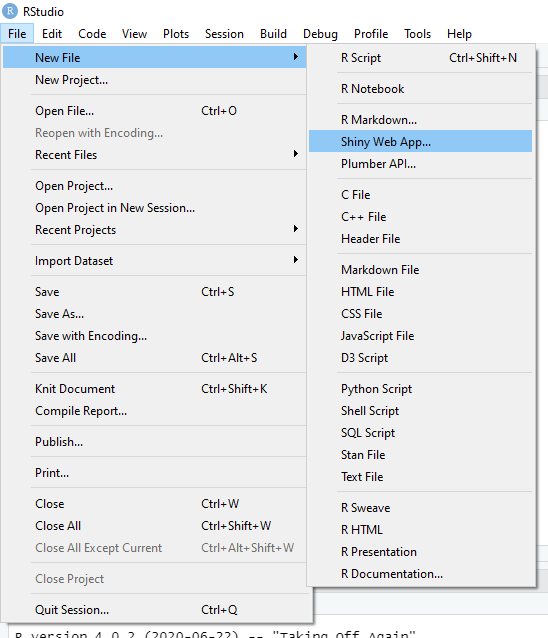
\includegraphics{./imagens/cap10imagem1.png}
\caption{Caminho para a criação do primeiro shiny}
\end{figure}

Irá aparecer a sua tela um popup que pedirá algumas configurações básicas. Veja abaixo:

\begin{itemize}
\tightlist
\item
  Application Name:

  \begin{itemize}
  \tightlist
  \item
    Esse é o nome da aplicação. O nome que você escolherá nessa hora só servirá para organização de pastas, portanto é importante se atentar a alguns detalhes:
  \item
    Sem caracteres especiais
  \item
    Escolha um nome explicativo, pois depois de um tempo vai ser muito dificil encontrar um projeto que tenha um nome genérico.
  \end{itemize}
\item
  Application type:

  \begin{itemize}
  \tightlist
  \item
    Aqui voce pode escolher uma entre duas opções: Single File ou Multiple File.
  \item
    Single File (app.R) vai gerar somente um arquivo chamado app.R. Essa é uma boa opção para shinys simples e com poucas linhas de código.
  \item
    Multiple File (ui.R/server.R) vai gerar dois arquivos. Um que vai conter o front-end (ui.R) e um para o back-end (server.R). É a melhor opção para quem gosta de códigos bem organizados e que gosta de criar apps mais completos. Neste tutorial vamos escolher essa opção.
  \end{itemize}
\item
  Create within directory:

  \begin{itemize}
  \tightlist
  \item
    Esse é o diretório que a pasta do shiny vai ser criada. É importante que nenhum das pastas que estão acima do app tenha caracteres especiais. Isso vai fazer com que você não consiga publicar seu aplicativo com facilidade.
  \end{itemize}
\end{itemize}

\begin{figure}
\centering
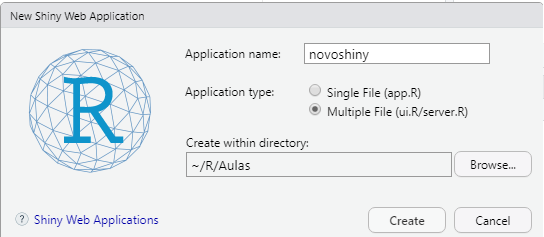
\includegraphics{./imagens/cap10imagem2.png}
\caption{Popup para criar o shiny}
\end{figure}

Com tudo isso em ordem, clique em ``Create''.

\hypertarget{ui-e-server}{%
\subsection{UI e SERVER}\label{ui-e-server}}

Com o shiny criado, dois arquivos serão gerados. O arquivo \texttt{ui.R} e o arquivo \texttt{server.R}.

\hypertarget{ui}{%
\subsubsection{UI}\label{ui}}

UI é sigla para User Interface. Isso significa que é nesse arquivo onde os elementos que serão visualizados pelo usuário do seu shiny irão estar dispostos. Neste arquivo não vamos fazer nenhuma manipulação de dados, análises, plots ou qualquer outra coisa que o valha. Iremos somente organizar a interface para que ela possa ser apresentada ao usuário final. Você deve encontrar algo similar a esse código no arquivo recém criado:

\begin{Shaded}
\begin{Highlighting}[]
\CommentTok{\#}
\CommentTok{\# This is the user{-}interface definition of a Shiny web application. You can}
\CommentTok{\# run the application by clicking \textquotesingle{}Run App\textquotesingle{} above.}
\CommentTok{\#}
\CommentTok{\# Find out more about building applications with Shiny here:}
\CommentTok{\#}
\CommentTok{\#    http://shiny.rstudio.com/}
\CommentTok{\#}

\FunctionTok{library}\NormalTok{(shiny)}

\CommentTok{\# Define UI for application that draws a histogram}
\FunctionTok{shinyUI}\NormalTok{(}\FunctionTok{fluidPage}\NormalTok{(}

    \CommentTok{\# Application title}
    \FunctionTok{titlePanel}\NormalTok{(}\StringTok{"Old Faithful Geyser Data"}\NormalTok{),}

    \CommentTok{\# Sidebar with a slider input for number of bins}
    \FunctionTok{sidebarLayout}\NormalTok{(}
        \FunctionTok{sidebarPanel}\NormalTok{(}
            \FunctionTok{sliderInput}\NormalTok{(}\StringTok{"bins"}\NormalTok{,}
                        \StringTok{"Number of bins:"}\NormalTok{,}
                        \AttributeTok{min =} \DecValTok{1}\NormalTok{,}
                        \AttributeTok{max =} \DecValTok{50}\NormalTok{,}
                        \AttributeTok{value =} \DecValTok{30}\NormalTok{)}
\NormalTok{        ),}

        \CommentTok{\# Show a plot of the generated distribution}
        \FunctionTok{mainPanel}\NormalTok{(}
            \FunctionTok{plotOutput}\NormalTok{(}\StringTok{"distPlot"}\NormalTok{)}
\NormalTok{        )}
\NormalTok{    )}
\NormalTok{))}
\end{Highlighting}
\end{Shaded}

Nele existem alguns elementos:

\begin{itemize}
\tightlist
\item
  Pacotes

  \begin{itemize}
  \tightlist
  \item
    Por convenção, os pacotes são sempre carregados no início do código. Neste caso, o unico pacote carregado é o \texttt{shiny} pois ele já tem os elementos necessários para criar seu primeiro shiny.
  \end{itemize}
\item
  \texttt{shinyUI()}

  \begin{itemize}
  \tightlist
  \item
    Essa função que gera a interface do usuário. É dentro dela que a gente vai passar como argumentos os elementos desta interface. Os elementos seguem nesta lista
  \item
    \texttt{fluidPage()} uma função que indica a criação de uma página flúida. Isso significa que esta página pode ser dividida em linhas e colunas. Cada linha tem largura fixa do tamanho da tela e altura alterável. Colunas existem para indicar quanto espaço horizontal dentro de um grid de 12 unidades cada elemento vai ocupar. Veremos esta disposição mais pra frente. Dentro dessa página existem outros elementos.
  \item
    \texttt{titlePanel()} título do painel. Será apresentado no início da página.
  \item
    \texttt{sidebarLayout()} indica que irá existir uma barra lateral e define seu layout.
  \item
    \texttt{sidebarPanel()} indica que a barra lateral será um painel flutuante.
  \item
    \texttt{sliderInput()} shiny widget que é composto por uma barra deslizante. Entraremos em mais detalhes do que são shiny widgets no futuro.
  \item
    \texttt{mainPanel()} painel que fica ao lado da barra lateral. É nele que os resultados serão mostrados, caso sejam passados como argumentos.
  \item
    \texttt{plotOutput()} indica que um gráfico está sendo gerado no servidor e que será incluído na interface de usuário onde essa função está sendo passada. Aceita o nome do plot indicado no servidor. Trataremos disto no futuro.
  \end{itemize}
\end{itemize}

\hypertarget{server}{%
\subsubsection{Server}\label{server}}

Esse arquivo é que vai conter todo o processamento dos dados que o seu aplicativo vai fazer. Todos os cálculos, gráficos e análises ficam aqui, e são referenciados para a interface do usuário. Ao criar o seu shiny, deve encontrar uma estrutura como essa no arquivo \texttt{server.R}:

\begin{Shaded}
\begin{Highlighting}[]
\CommentTok{\#}
\CommentTok{\# This is the server logic of a Shiny web application. You can run the}
\CommentTok{\# application by clicking \textquotesingle{}Run App\textquotesingle{} above.}
\CommentTok{\#}
\CommentTok{\# Find out more about building applications with Shiny here:}
\CommentTok{\#}
\CommentTok{\#    http://shiny.rstudio.com/}
\CommentTok{\#}

\FunctionTok{library}\NormalTok{(shiny)}

\CommentTok{\# Define server logic required to draw a histogram}
\FunctionTok{shinyServer}\NormalTok{(}\ControlFlowTok{function}\NormalTok{(input, output) \{}

\NormalTok{    output}\SpecialCharTok{$}\NormalTok{distPlot }\OtherTok{\textless{}{-}} \FunctionTok{renderPlot}\NormalTok{(\{}

        \CommentTok{\# generate bins based on input$bins from ui.R}
\NormalTok{        x    }\OtherTok{\textless{}{-}}\NormalTok{ faithful[, }\DecValTok{2}\NormalTok{]}
\NormalTok{        bins }\OtherTok{\textless{}{-}} \FunctionTok{seq}\NormalTok{(}\FunctionTok{min}\NormalTok{(x), }\FunctionTok{max}\NormalTok{(x), }\AttributeTok{length.out =}\NormalTok{ input}\SpecialCharTok{$}\NormalTok{bins }\SpecialCharTok{+} \DecValTok{1}\NormalTok{)}

        \CommentTok{\# draw the histogram with the specified number of bins}
        \FunctionTok{hist}\NormalTok{(x, }\AttributeTok{breaks =}\NormalTok{ bins, }\AttributeTok{col =} \StringTok{\textquotesingle{}darkgray\textquotesingle{}}\NormalTok{, }\AttributeTok{border =} \StringTok{\textquotesingle{}white\textquotesingle{}}\NormalTok{)}

\NormalTok{    \})}

\NormalTok{\})}
\end{Highlighting}
\end{Shaded}

Os elementos são os que seguem:

\begin{itemize}
\tightlist
\item
  Pacotes

  \begin{itemize}
  \tightlist
  \item
    Os pacotes sao carregados sempre no começo e fora da função \texttt{shinyServer()}. Caso coloque dentro desta função, os pacotes serão carregados sempre que houver qualquer interação do usuário com o aplicativo.
  \end{itemize}
\item
  \texttt{shinyServer()}

  \begin{itemize}
  \tightlist
  \item
    Essa função é que indica que aqui estão os elementos que compõem o backend (cálculos, plots e afins). Ela recebe alguns argumentos, dois listados abaixo e outros que não veremos neste livro.
  \item
    input - tudo que vem da interface do usuário, capturados pelos shiny widgets. Veremos mais sobre shiny widgets no futuro.
  \item
    output - tudo que sai do servidor e vai ser utilizado na interface do usuário. É um objeto que contém vários outros objetos.
  \end{itemize}
\end{itemize}

A função \texttt{shinyServer()} recebe uma função dentro dela, e permite a abertura de um bloco de código, apontados pelas \texttt{\{\}}. Dentro dela podemos atribuir ao objeto \texttt{output} os elementos que serão apresentados na interface de usuário. O exemplo acima faz isso com o elemento distPlot. Vamos entender o que ele significa:

\begin{itemize}
\tightlist
\item
  \texttt{output\$distPlot\ \textless{}-} esse código significa que o \texttt{output} vai conter um objeto chamado \texttt{distplot}. Logo em seguida existe o \texttt{\textless{}-}, que indica atribuição de objeto.
\item
  \texttt{renderPlot(\{\})} esse comando indica que o que vai ficar salvo em \texttt{output\$distPlot} é um plot renderizado. Ou seja, um plot que pode ser aberto em uma página da internet. Como está em um bloco de código, o exemplo atribui alguns valores e vetores a objetos e plota um histograma. Normalmente esse plot seria apresentado no proprio RStudio, mas como estamos tratando de um shiny, esse plot será enviado a interface do usuário e será apresentado onde a função \texttt{plotOutput("distPlot")} está inserida.
\end{itemize}

Ao clicar em \texttt{Run\ App} o seu shiny será gerado. Esse botão está nessa localização:

\begin{figure}
\centering
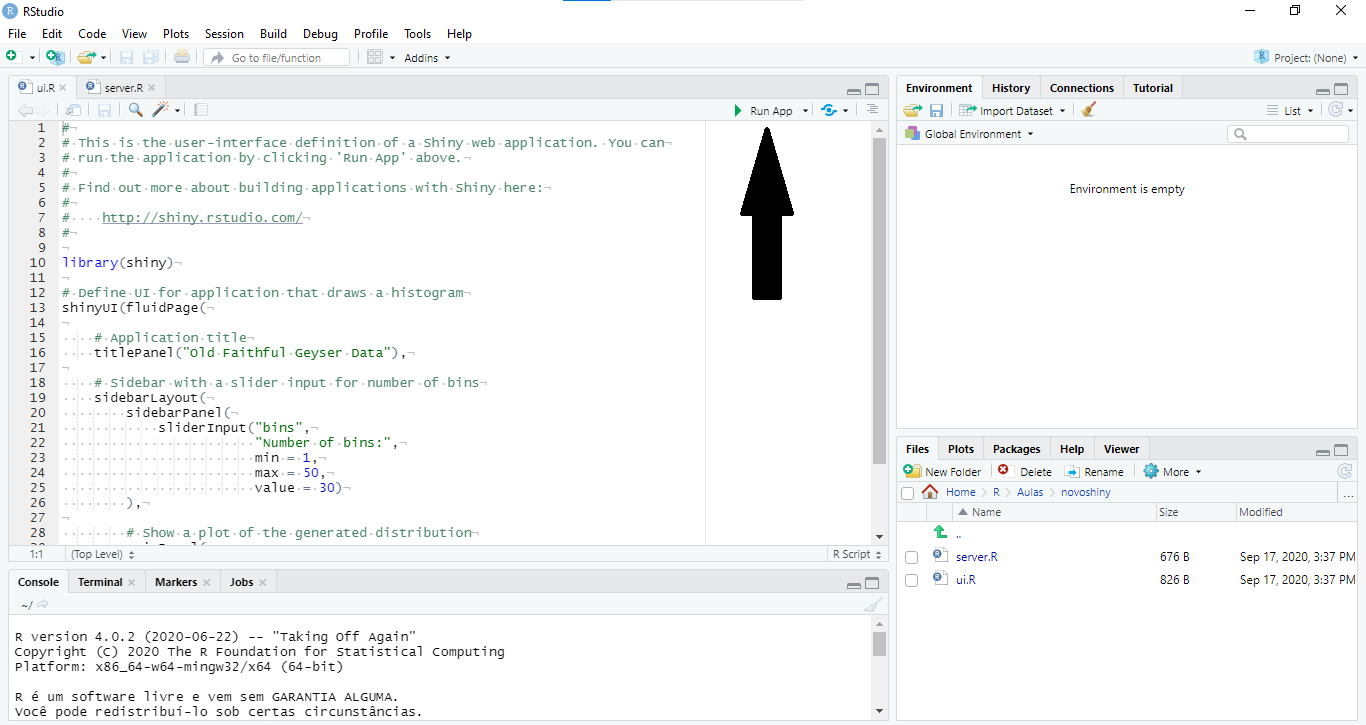
\includegraphics{./imagens/cap10imagem4.png}
\caption{Botão Run App}
\end{figure}

Ao clicar, você deve ter encontrado uma página como essa:

\begin{figure}
\centering
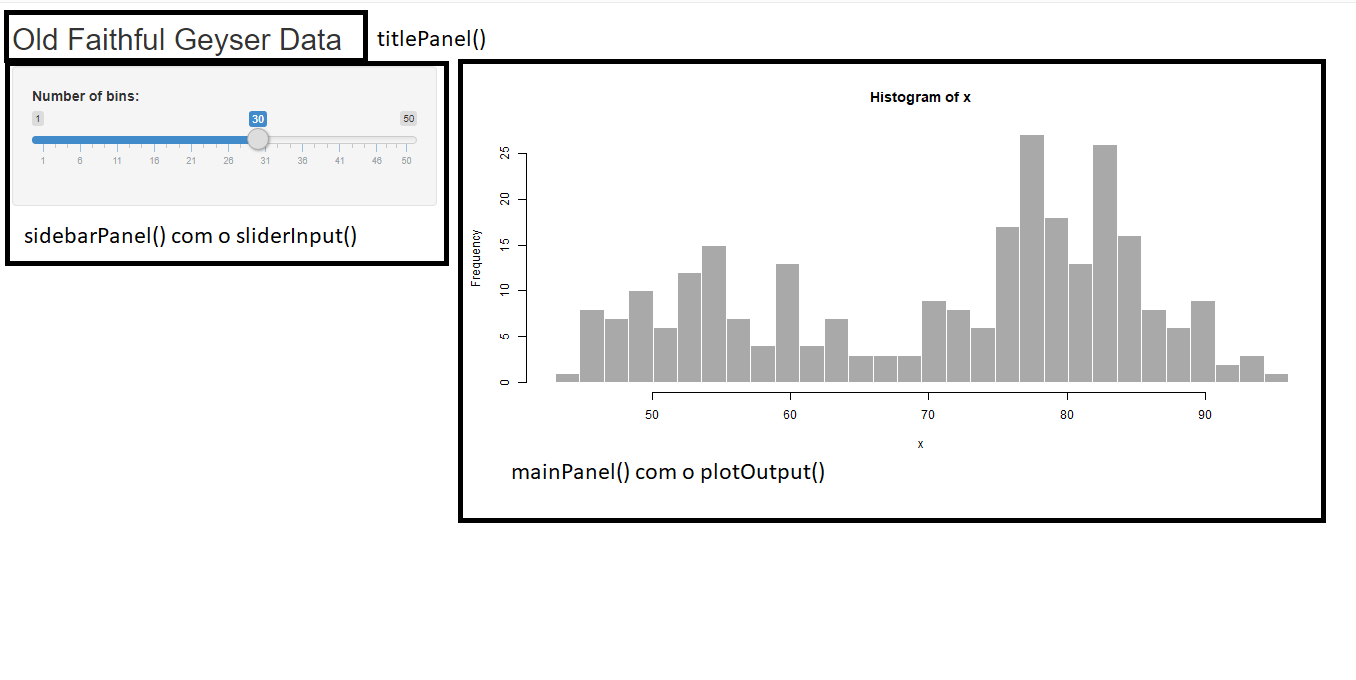
\includegraphics{./imagens/cap10imagem5.png}
\caption{Exemplo de shiny}
\end{figure}

\hypertarget{shiny2}{%
\chapter{Avançando no Shiny}\label{shiny2}}

Agora que você já sabe o que é um shiny e como funciona sua estrutura, vamos criar nossa primeira dashboard! Esse é um modelo de visualização de dados bem aceito no mercado, o que torna esse aprendizado muito útil pra um profissional que está buscando cargos de análise de dados ou psicometria.

Antes de tudo, vamos limpar os arquivos \texttt{ui.R} e \texttt{server.R}. Já vamos inserir a estrutura que o pacote \texttt{shinydashboard} sugere.

\emph{UI}

\begin{Shaded}
\begin{Highlighting}[]
\FunctionTok{library}\NormalTok{(shinydashboard) }\CommentTok{\# instale, caso não tenha instalado}

\FunctionTok{dashboardPage}\NormalTok{(}
  \FunctionTok{dashboardHeader}\NormalTok{(),}
  \FunctionTok{dashboardSidebar}\NormalTok{(),}
  \FunctionTok{dashboardBody}\NormalTok{()}
\NormalTok{)}
\end{Highlighting}
\end{Shaded}

\emph{SERVER}

\begin{Shaded}
\begin{Highlighting}[]
\FunctionTok{library}\NormalTok{(shiny)}

\FunctionTok{shinyServer}\NormalTok{(}\ControlFlowTok{function}\NormalTok{(input, output) \{}

\NormalTok{\})}
\end{Highlighting}
\end{Shaded}

Ao rodar o aplicativo pelo botão \texttt{Run\ App} você deverá ter um shiny assim:

\begin{figure}
\centering
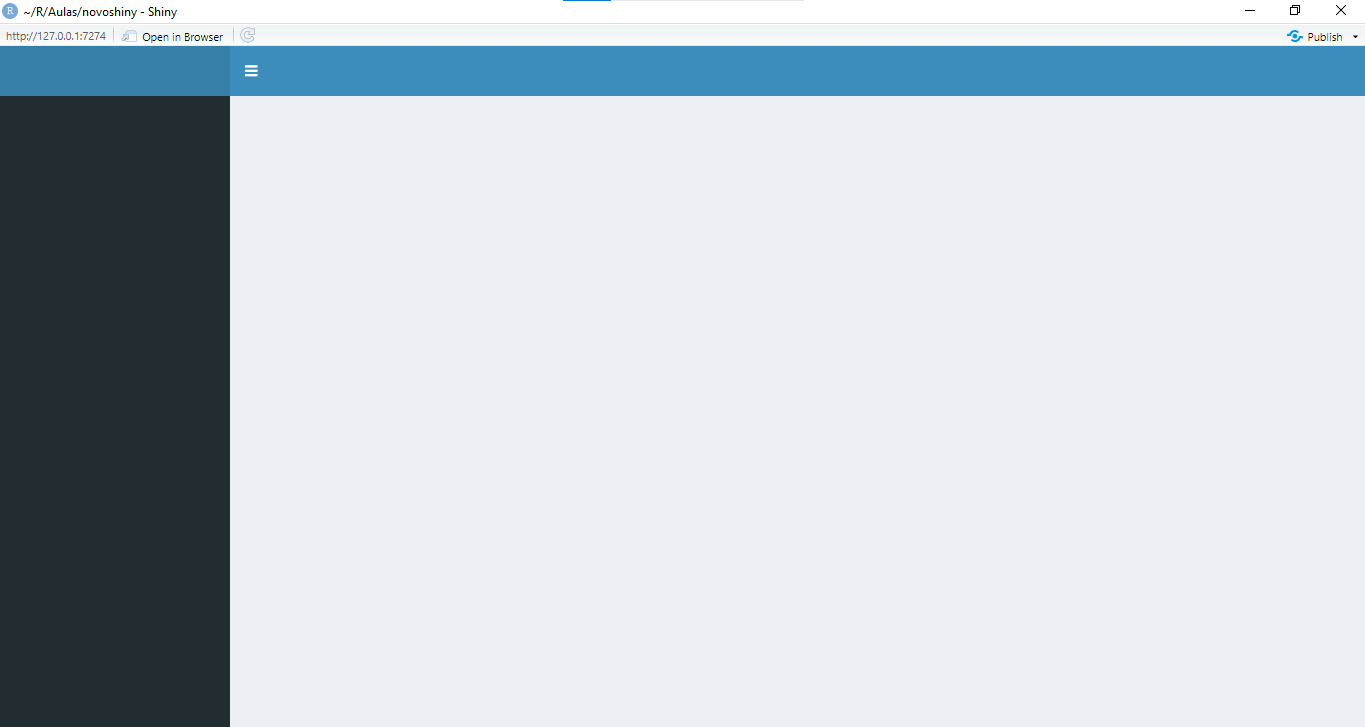
\includegraphics{./imagens/cap10imagem6.png}
\caption{Shiny dashboard}
\end{figure}

\hypertarget{manipulando-elementos-do-ui}{%
\section{Manipulando elementos do UI}\label{manipulando-elementos-do-ui}}

\hypertarget{tuxedtulo-e-sidebar}{%
\subsection{Título e sidebar}\label{tuxedtulo-e-sidebar}}

Para adicionar um título ao seu shiny, vamos passar o argumento \texttt{title\ =} na função \texttt{dashboardHeader()} no \texttt{ui.R}.

\begin{Shaded}
\begin{Highlighting}[]
\FunctionTok{library}\NormalTok{(shinydashboard)}

\FunctionTok{dashboardPage}\NormalTok{(}
  \FunctionTok{dashboardHeader}\NormalTok{(}
    \AttributeTok{title =} \StringTok{\textquotesingle{}Meu primeiro Shiny\textquotesingle{}}
\NormalTok{  ),}
  \FunctionTok{dashboardSidebar}\NormalTok{(),}
  \FunctionTok{dashboardBody}\NormalTok{()}
\NormalTok{)}
\end{Highlighting}
\end{Shaded}

O resultado será esse:

\begin{figure}
\centering
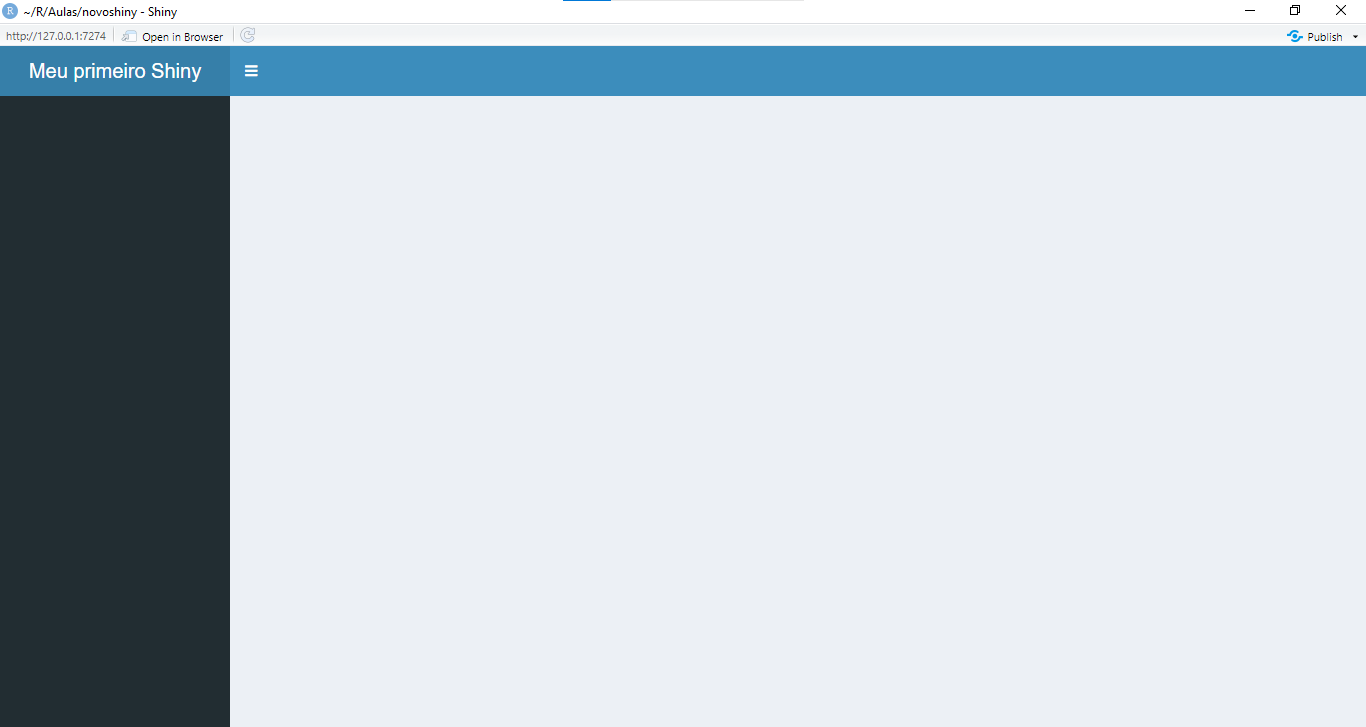
\includegraphics{./imagens/cap10imagem7.png}
\caption{Alterando título}
\end{figure}

Caso você dê um título muito grande, será preciso aumentar a largura do \texttt{Header}. Para isso, passe argumento \texttt{titleWidth\ =}. Ele aceita um número em pixel, como o exemplo abaixo, ou um valor em percentagem passado dentro de aspas duplas, como \texttt{titleWidth\ =\ "20\%"}. Siga o exemplo abaixo.

\begin{Shaded}
\begin{Highlighting}[]
\FunctionTok{library}\NormalTok{(shinydashboard)}

\FunctionTok{dashboardPage}\NormalTok{(}
  \FunctionTok{dashboardHeader}\NormalTok{(}
    \AttributeTok{title =} \StringTok{\textquotesingle{}Meu primeiro Shiny feito com carinho\textquotesingle{}}\NormalTok{,}
    \AttributeTok{titleWidth =} \DecValTok{400}
\NormalTok{  ),}
  \FunctionTok{dashboardSidebar}\NormalTok{(),}
  \FunctionTok{dashboardBody}\NormalTok{()}
\NormalTok{)}
\end{Highlighting}
\end{Shaded}

O resultado será esse:

\begin{figure}
\centering
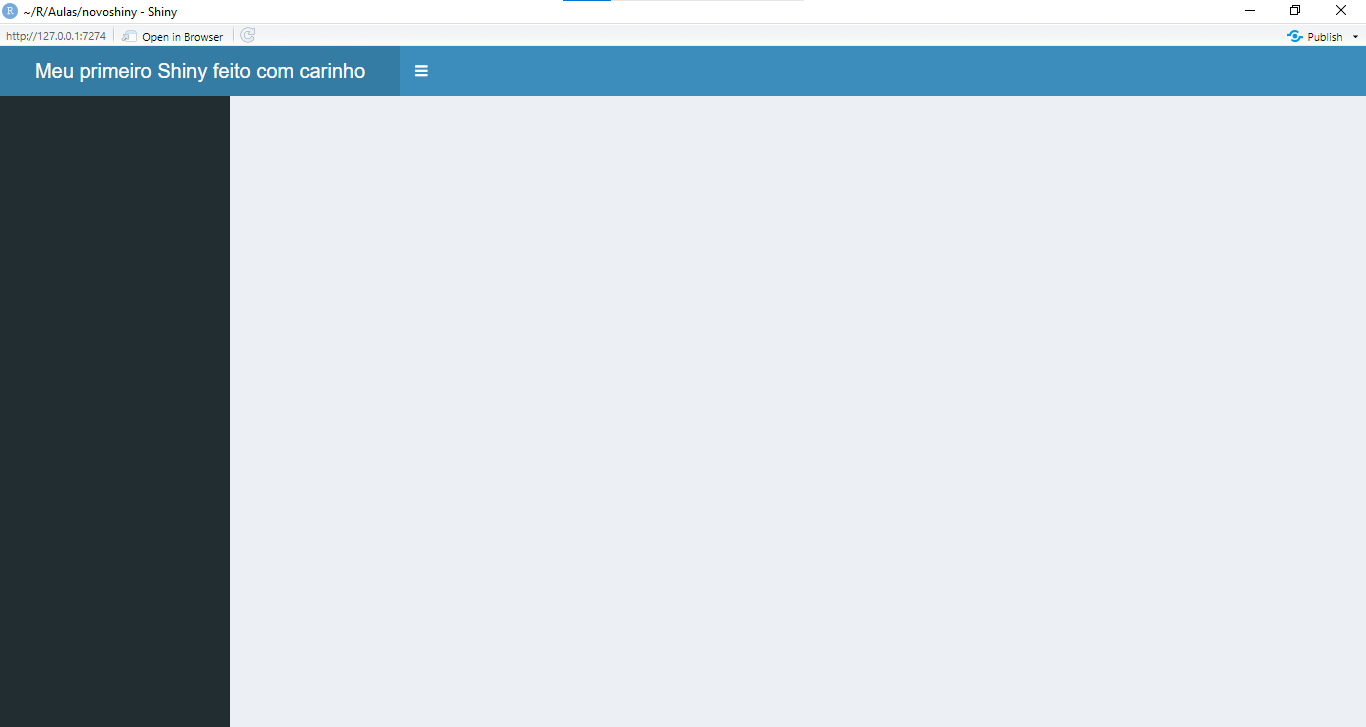
\includegraphics{./imagens/cap10imagem8.png}
\caption{Alterando largura do Header}
\end{figure}

A largura da \texttt{sidebar} também pode ser alterada ao passar o argumento \texttt{width\ =} na função \texttt{dashboardSidebar()}. Veja:

\begin{Shaded}
\begin{Highlighting}[]
\FunctionTok{library}\NormalTok{(shinydashboard)}

\FunctionTok{dashboardPage}\NormalTok{(}
  \FunctionTok{dashboardHeader}\NormalTok{(}
    \AttributeTok{title =} \StringTok{\textquotesingle{}Meu primeiro Shiny feito com carinho\textquotesingle{}}\NormalTok{,}
    \AttributeTok{titleWidth =} \DecValTok{400}
\NormalTok{  ),}
  \FunctionTok{dashboardSidebar}\NormalTok{(}
    \AttributeTok{width =} \DecValTok{400}
\NormalTok{  ),}
  \FunctionTok{dashboardBody}\NormalTok{()}
\NormalTok{)}
\end{Highlighting}
\end{Shaded}

\begin{figure}
\centering
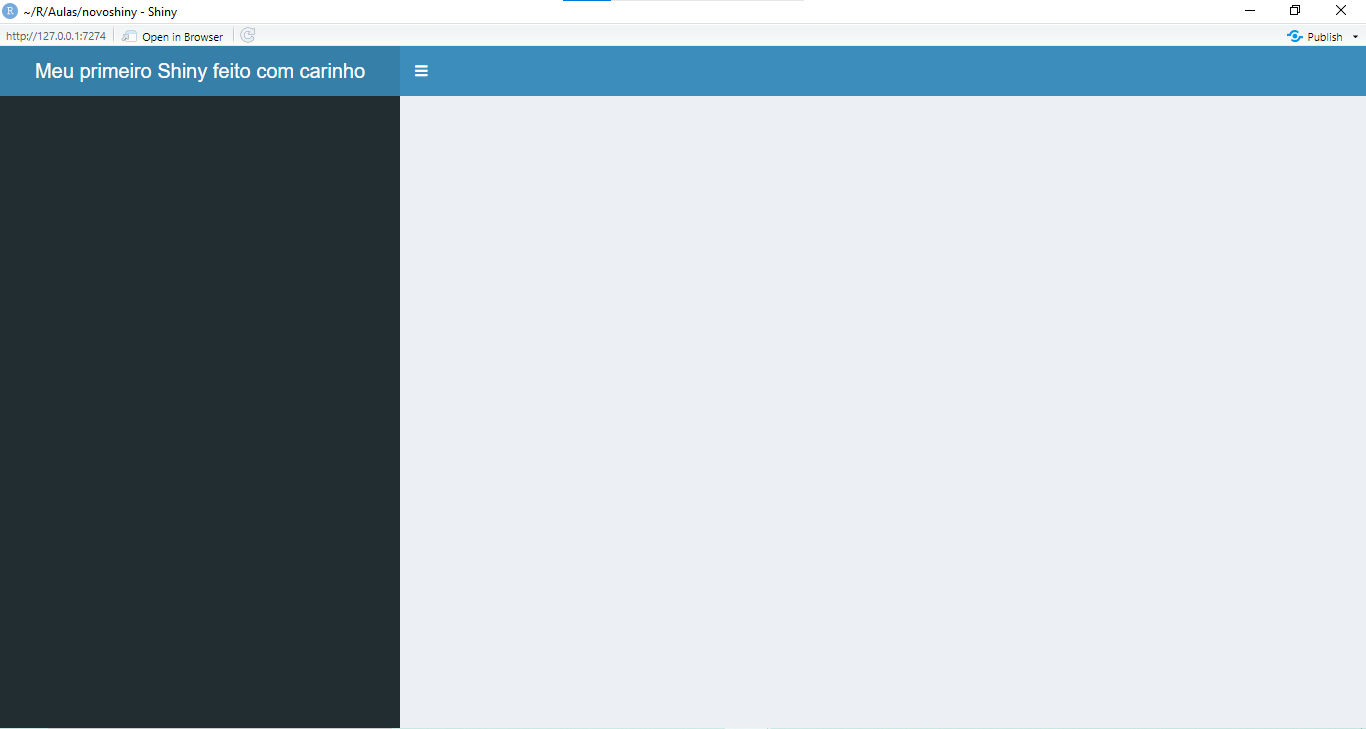
\includegraphics{./imagens/cap10imagem9.png}
\caption{Alterando largura da sidebar}
\end{figure}

\hypertarget{body}{%
\subsection{Body}\label{body}}

Para incluir algum elemento no corpo do shiny, basta passar como argumento dentro de \texttt{dashboardBody()}. Vamos apresentar alguns elementos de texto que podem ser úteis no futuro.

\begin{itemize}
\tightlist
\item
  \texttt{h1()} até \texttt{h5()}

  \begin{itemize}
  \tightlist
  \item
    Estas funções adicionam títulos, basta passar um texto entre aspas.
  \end{itemize}
\item
  \texttt{p()}

  \begin{itemize}
  \tightlist
  \item
    Função que adiciona um parágrafo.
  \end{itemize}
\item
  \texttt{br()}

  \begin{itemize}
  \tightlist
  \item
    Função que pula linha
  \end{itemize}
\end{itemize}

Vamos testar em nosso shiny?

\begin{Shaded}
\begin{Highlighting}[]
\FunctionTok{library}\NormalTok{(shinydashboard)}

\FunctionTok{dashboardPage}\NormalTok{(}
  \FunctionTok{dashboardHeader}\NormalTok{(}
    \AttributeTok{title =} \StringTok{\textquotesingle{}Meu primeiro Shiny feito com carinho\textquotesingle{}}\NormalTok{,}
    \AttributeTok{titleWidth =} \DecValTok{400}
\NormalTok{  ),}
  \FunctionTok{dashboardSidebar}\NormalTok{(}
    \AttributeTok{width =} \DecValTok{400}
\NormalTok{  ),}
  \FunctionTok{dashboardBody}\NormalTok{(}
    \FunctionTok{h1}\NormalTok{(}\StringTok{\textquotesingle{}Título 1\textquotesingle{}}\NormalTok{),}
    \FunctionTok{h3}\NormalTok{(}\StringTok{\textquotesingle{}Título 3\textquotesingle{}}\NormalTok{),}
    \FunctionTok{h5}\NormalTok{(}\StringTok{\textquotesingle{}Título 5\textquotesingle{}}\NormalTok{),}
    \FunctionTok{br}\NormalTok{(),}
    \FunctionTok{p}\NormalTok{(}\StringTok{\textquotesingle{}Parágrafo\textquotesingle{}}\NormalTok{)}
\NormalTok{  )}
\NormalTok{)}
\end{Highlighting}
\end{Shaded}

Veja o resultado:

\begin{figure}
\centering
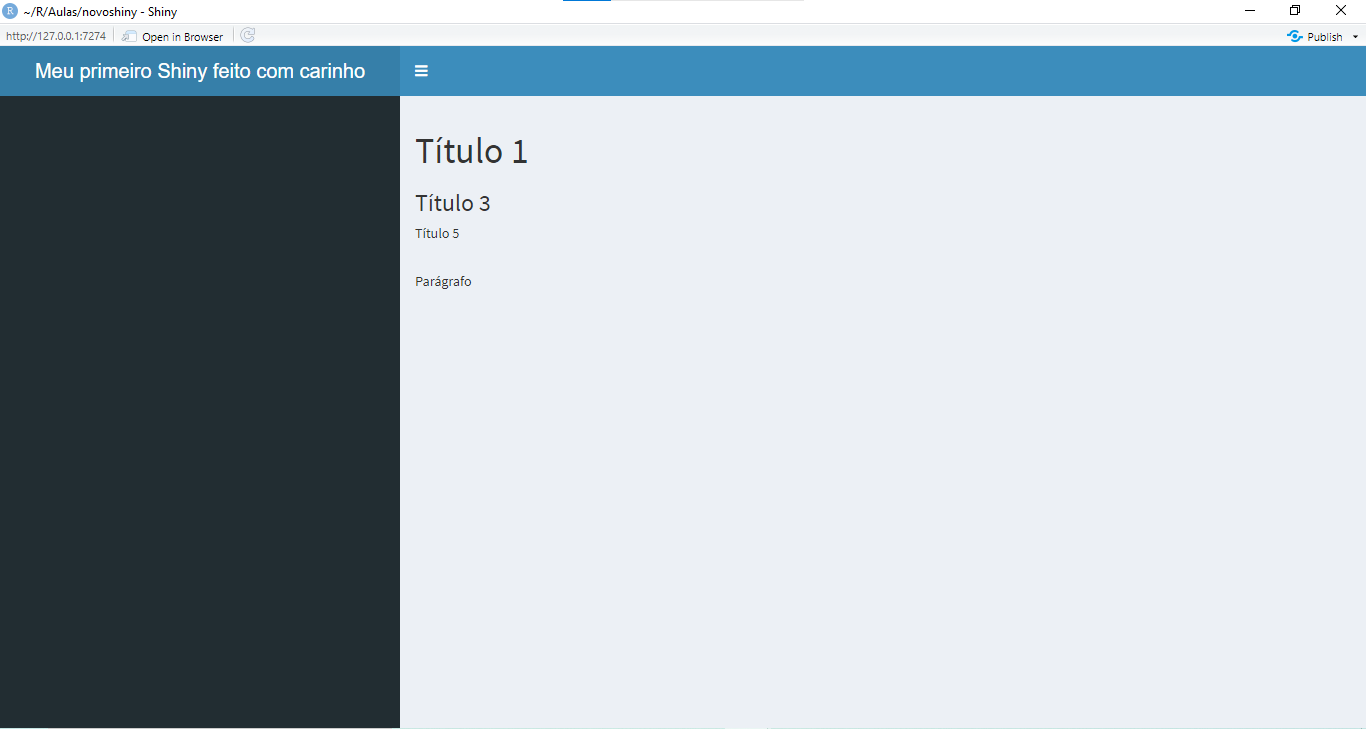
\includegraphics{./imagens/cap10imagem10.png}
\caption{Elementos no body}
\end{figure}

Antes de seguir adiante, limpe o \texttt{ui.R} para facilitar nosso entendimento:

\begin{Shaded}
\begin{Highlighting}[]
\FunctionTok{library}\NormalTok{(shinydashboard)}

\FunctionTok{dashboardPage}\NormalTok{(}
  \FunctionTok{dashboardHeader}\NormalTok{(}
    \AttributeTok{title =} \StringTok{\textquotesingle{}Meu primeiro Shiny\textquotesingle{}}
\NormalTok{  ),}
  \FunctionTok{dashboardSidebar}\NormalTok{(),}
  \FunctionTok{dashboardBody}\NormalTok{()}
\NormalTok{)}
\end{Highlighting}
\end{Shaded}

\hypertarget{ui-e-server-trabalhando-juntos}{%
\section{Ui e Server trabalhando juntos}\label{ui-e-server-trabalhando-juntos}}

\hypertarget{tabela}{%
\subsection{Tabela}\label{tabela}}

Conforme foi visto no capítulo anterior, é preciso atribuir ao objeto \texttt{output} no \texttt{server} para que seja possível apresentá-lo na \texttt{ui}. Agora nós vamos aprender como apresentar tabelas no nosso shiny.

Primeiro, não esqueça de carregar os objetos que a gente precisa com o \texttt{load(\textquotesingle{}bases.RData\textquotesingle{})}. Depois, nós vamos anexar ao \texttt{output} a renderização e uma tabela, com o nome de \texttt{tabela}. \texttt{renderTable()} irá preparar uma tabela normalmente apresentada no console para que possa ser apresentada no shiny. Em \texttt{renderTable()} vamos passar o dataframe \texttt{db}

Depois, vamos pedir que essa tabela seja apresentada no \texttt{ui}com \texttt{tableOutput()}. Veja como ficam os arquivos.

\emph{UI}

\begin{Shaded}
\begin{Highlighting}[]
\FunctionTok{library}\NormalTok{(shinydashboard)}

\FunctionTok{dashboardPage}\NormalTok{(}
  \FunctionTok{dashboardHeader}\NormalTok{(}
    \AttributeTok{title =} \StringTok{\textquotesingle{}Meu primeiro Shiny\textquotesingle{}}
\NormalTok{  ),}
  \FunctionTok{dashboardSidebar}\NormalTok{(),}
  \FunctionTok{dashboardBody}\NormalTok{(}
    \FunctionTok{tableOutput}\NormalTok{(}\StringTok{\textquotesingle{}tabela\textquotesingle{}}\NormalTok{)}
\NormalTok{  )}
\NormalTok{)}
\end{Highlighting}
\end{Shaded}

\emph{SERVER}

\begin{Shaded}
\begin{Highlighting}[]
\FunctionTok{library}\NormalTok{(shiny)}

\FunctionTok{load}\NormalTok{(}\StringTok{\textquotesingle{}bases.RData\textquotesingle{}}\NormalTok{) }\CommentTok{\# carregamos fora da função shinyserver pra ser carregado somente uma vez}

\FunctionTok{shinyServer}\NormalTok{(}\ControlFlowTok{function}\NormalTok{(input, output) \{}

\NormalTok{  output}\SpecialCharTok{$}\NormalTok{tabela }\OtherTok{\textless{}{-}} \FunctionTok{renderTable}\NormalTok{(db)}

\NormalTok{\})}
\end{Highlighting}
\end{Shaded}

O resultado será esse:

\begin{figure}
\centering
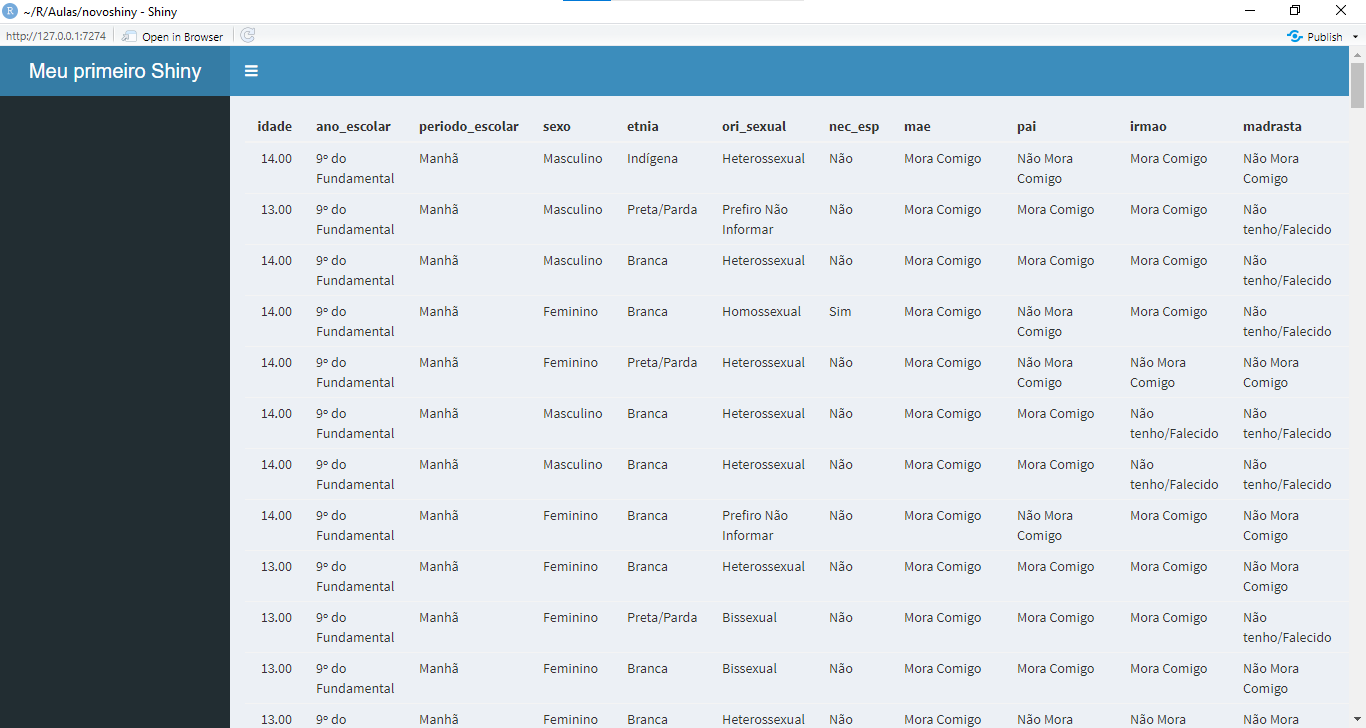
\includegraphics{./imagens/cap10imagem11.png}
\caption{Tabela}
\end{figure}

\hypertarget{datatable}{%
\subsection{Datatable}\label{datatable}}

Alguns problemas ficaram evidentes. Primeiro, que a tabela é muito grande e muito larga, o que impede sua visualização. O segundo problema é que essa tabela não ajuda muito a explração dos dados. Para tentar resolver esses problemas vamos usar a função \texttt{renderDataTable()}, com dois argumentos: a base de dados e \texttt{options\ =} que recebe uma lista com as opções que queremos passar. Aqui, vamos pedir que haja barra de rolagem no eixo x com \texttt{scrollX\ =\ TRUE} e limitar o máximo de observações por página a 5, com \texttt{pageLength\ =\ 5}. Também precisaremos alterar o \texttt{ui} para receber esse tipo de tabela, trocando \texttt{tableOutput()} por \texttt{dataTableOutput()}. Veja como ficam os arquivos:

\begin{Shaded}
\begin{Highlighting}[]
\FunctionTok{library}\NormalTok{(shinydashboard)}

\FunctionTok{dashboardPage}\NormalTok{(}
  \FunctionTok{dashboardHeader}\NormalTok{(}
    \AttributeTok{title =} \StringTok{\textquotesingle{}Meu primeiro Shiny\textquotesingle{}}
\NormalTok{  ),}
  \FunctionTok{dashboardSidebar}\NormalTok{(),}
  \FunctionTok{dashboardBody}\NormalTok{(}
    \FunctionTok{dataTableOutput}\NormalTok{(}\StringTok{\textquotesingle{}tabela\textquotesingle{}}\NormalTok{)}
\NormalTok{  )}
\NormalTok{)}
\end{Highlighting}
\end{Shaded}

\emph{SERVER}

\begin{Shaded}
\begin{Highlighting}[]
\FunctionTok{library}\NormalTok{(shiny)}

\FunctionTok{load}\NormalTok{(}\StringTok{\textquotesingle{}bases.RData\textquotesingle{}}\NormalTok{) }\CommentTok{\# carregamos fora da função shinyserver pra ser carregado somente uma vez}

\FunctionTok{shinyServer}\NormalTok{(}\ControlFlowTok{function}\NormalTok{(input, output) \{}

\NormalTok{  output}\SpecialCharTok{$}\NormalTok{tabela }\OtherTok{\textless{}{-}} \FunctionTok{renderDataTable}\NormalTok{(}
\NormalTok{  db,}
  \AttributeTok{options =} \FunctionTok{list}\NormalTok{(}
    \AttributeTok{scrollX =} \ConstantTok{TRUE}\NormalTok{,}
    \AttributeTok{pageLength =} \DecValTok{5}
\NormalTok{  )}
\NormalTok{)}

\NormalTok{\})}
\end{Highlighting}
\end{Shaded}

O resultado será esse:

\begin{figure}
\centering
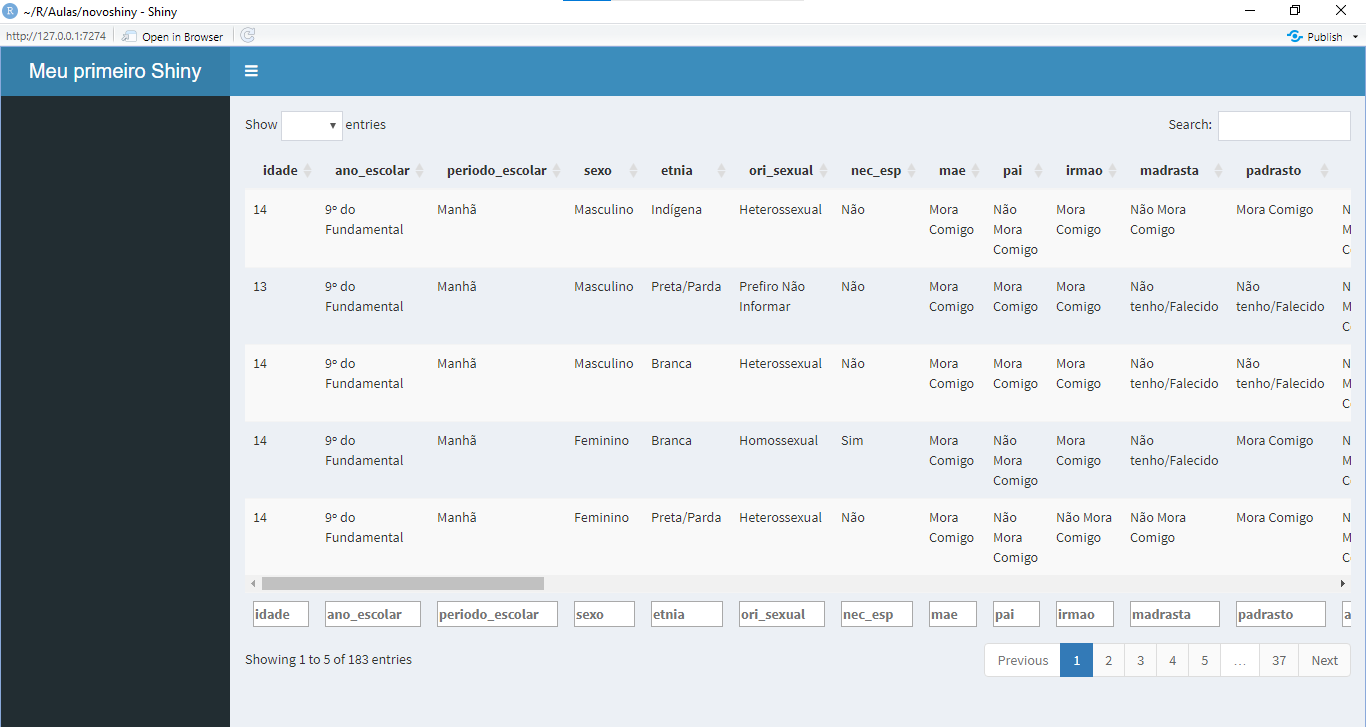
\includegraphics{./imagens/cap10imagem12.png}
\caption{Datatable}
\end{figure}

\hypertarget{menu-itens}{%
\section{Menu itens}\label{menu-itens}}

Normalmente essas dashboards sempre apresentam tipos diferentes de dados. Para isso a gente precisa organizar melhor nossa parte visual. Por enquanto vamos alterar somente o \texttt{ui.R}.

A função \texttt{dashboardSidebar()} pode receber város argumentos e outras funções. Entre elas, a função \texttt{sidebarMenu()} permite que você crie itens de menu que ao serem clicados carregam um \texttt{body} diferente. Para isso, basta chamar a função \texttt{menuItem()}, que receberá dois argumentos: O primeiro é o que estará escrito nela, e o segundo, \texttt{tabName\ =}, o nome que será usado para identificar esse \texttt{menuItem}.

No entanto, para isso funcionar precisaremos passar a função \texttt{tabItens()} ao \texttt{dashboardBody()}. Essa função recebe como argumentos a função \texttt{tabItem()} que faz o link com o \texttt{meuItem()} explicado anteriormente. O primeiro argumento que ela recebe é sempre \texttt{tabName\ =}, que deve conter o mesmo nome identificado em \texttt{menuItem}, no argumento de mesmo nome. Após isso, trate como se fosse um \texttt{body} normal.

Veja esse exemplo:

\begin{Shaded}
\begin{Highlighting}[]
\FunctionTok{library}\NormalTok{(shinydashboard)}

\FunctionTok{dashboardPage}\NormalTok{(}
  \FunctionTok{dashboardHeader}\NormalTok{(}
    \AttributeTok{title =} \StringTok{\textquotesingle{}Meu primeiro Shiny\textquotesingle{}}
\NormalTok{  ),}
  \FunctionTok{dashboardSidebar}\NormalTok{(}
    \FunctionTok{sidebarMenu}\NormalTok{(}
      \FunctionTok{menuItem}\NormalTok{(}\StringTok{"Base de dados"}\NormalTok{, }\AttributeTok{tabName =} \StringTok{"basededados"}\NormalTok{)}
\NormalTok{    )}
\NormalTok{  ),}
  \FunctionTok{dashboardBody}\NormalTok{(}
    \FunctionTok{tabItems}\NormalTok{(}
      \FunctionTok{tabItem}\NormalTok{(}
        \AttributeTok{tabName =} \StringTok{"basededados"}\NormalTok{,}
        \FunctionTok{h2}\NormalTok{(}\StringTok{"Base de dados"}\NormalTok{),}
        \FunctionTok{dataTableOutput}\NormalTok{(}\StringTok{\textquotesingle{}tabela\textquotesingle{}}\NormalTok{)}
\NormalTok{      )}
\NormalTok{    )}
\NormalTok{  )}
\NormalTok{)}
\end{Highlighting}
\end{Shaded}

O resultado é esse:

\begin{figure}
\centering
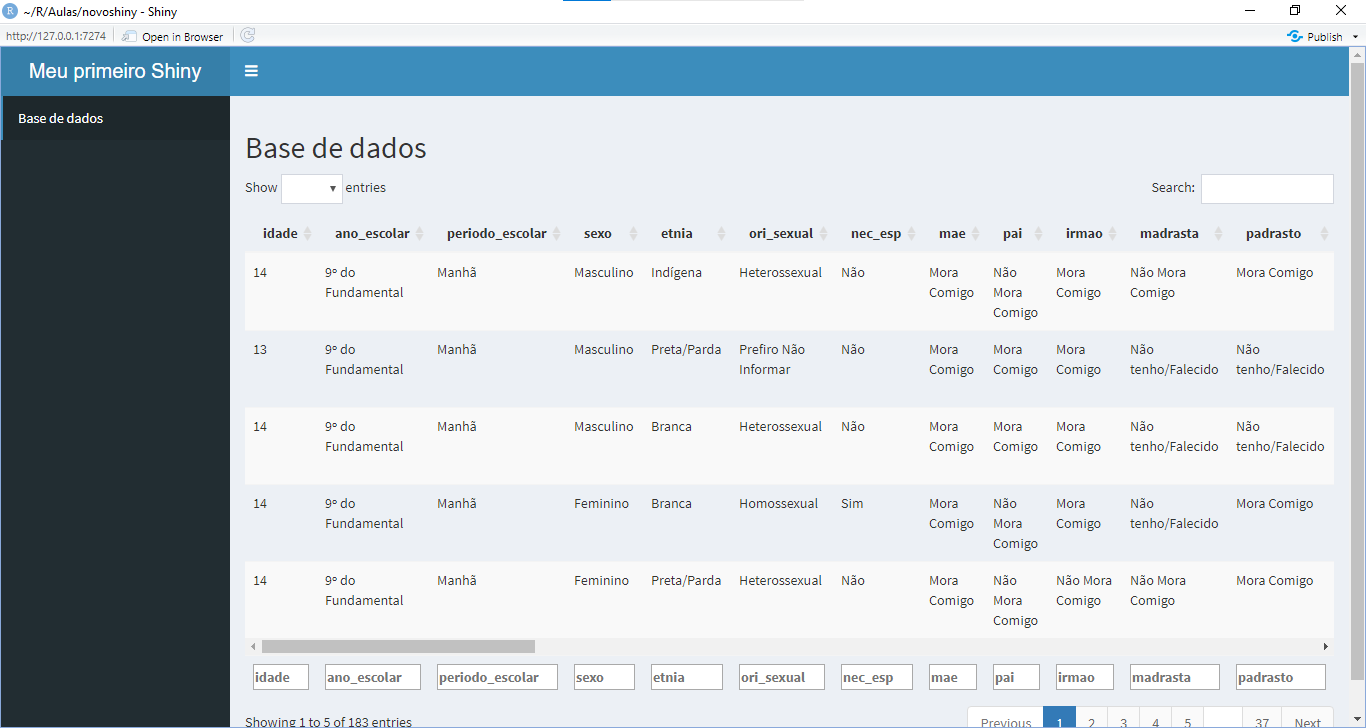
\includegraphics{./imagens/cap10imagem13.png}
\caption{Datatable}
\end{figure}

Agora vamos preparar mais um menu para incluir um gráfico que iremos produzir a seguir. Crie outro \texttt{menuItem} na \texttt{sidebar} e outro \texttt{tabItem} no \texttt{body}.

\begin{Shaded}
\begin{Highlighting}[]
\FunctionTok{library}\NormalTok{(shinydashboard)}

\FunctionTok{dashboardPage}\NormalTok{(}
  \FunctionTok{dashboardHeader}\NormalTok{(}
    \AttributeTok{title =} \StringTok{\textquotesingle{}Meu primeiro Shiny\textquotesingle{}}
\NormalTok{  ),}
  \FunctionTok{dashboardSidebar}\NormalTok{(}
    \FunctionTok{sidebarMenu}\NormalTok{(}
      \FunctionTok{menuItem}\NormalTok{(}\StringTok{\textquotesingle{}Base de dados\textquotesingle{}}\NormalTok{, }\AttributeTok{tabName =} \StringTok{\textquotesingle{}basededados\textquotesingle{}}\NormalTok{),}
      \FunctionTok{menuItem}\NormalTok{(}\StringTok{\textquotesingle{}Plots\textquotesingle{}}\NormalTok{, }\AttributeTok{tabName =} \StringTok{\textquotesingle{}plots\textquotesingle{}}\NormalTok{)}
\NormalTok{    )}
\NormalTok{  ),}
  \FunctionTok{dashboardBody}\NormalTok{(}
    \FunctionTok{tabItems}\NormalTok{(}
      \FunctionTok{tabItem}\NormalTok{(}
        \AttributeTok{tabName =} \StringTok{\textquotesingle{}basededados\textquotesingle{}}\NormalTok{,}
        \FunctionTok{h1}\NormalTok{(}\StringTok{\textquotesingle{}Base de dados\textquotesingle{}}\NormalTok{),}
        \FunctionTok{dataTableOutput}\NormalTok{(}\StringTok{\textquotesingle{}tabela\textquotesingle{}}\NormalTok{)}
\NormalTok{      ),}
      \FunctionTok{tabItem}\NormalTok{(}
        \AttributeTok{tabName =} \StringTok{\textquotesingle{}plots\textquotesingle{}}\NormalTok{,}
        \FunctionTok{h1}\NormalTok{(}\StringTok{\textquotesingle{}Esses são os plots\textquotesingle{}}\NormalTok{)}
\NormalTok{      )}
\NormalTok{    )}
\NormalTok{  )}
\NormalTok{)}
\end{Highlighting}
\end{Shaded}

Explore o resultado e perceba o que acontece quando clica no item \texttt{Plots} da \texttt{sidebar}.

\begin{figure}
\centering
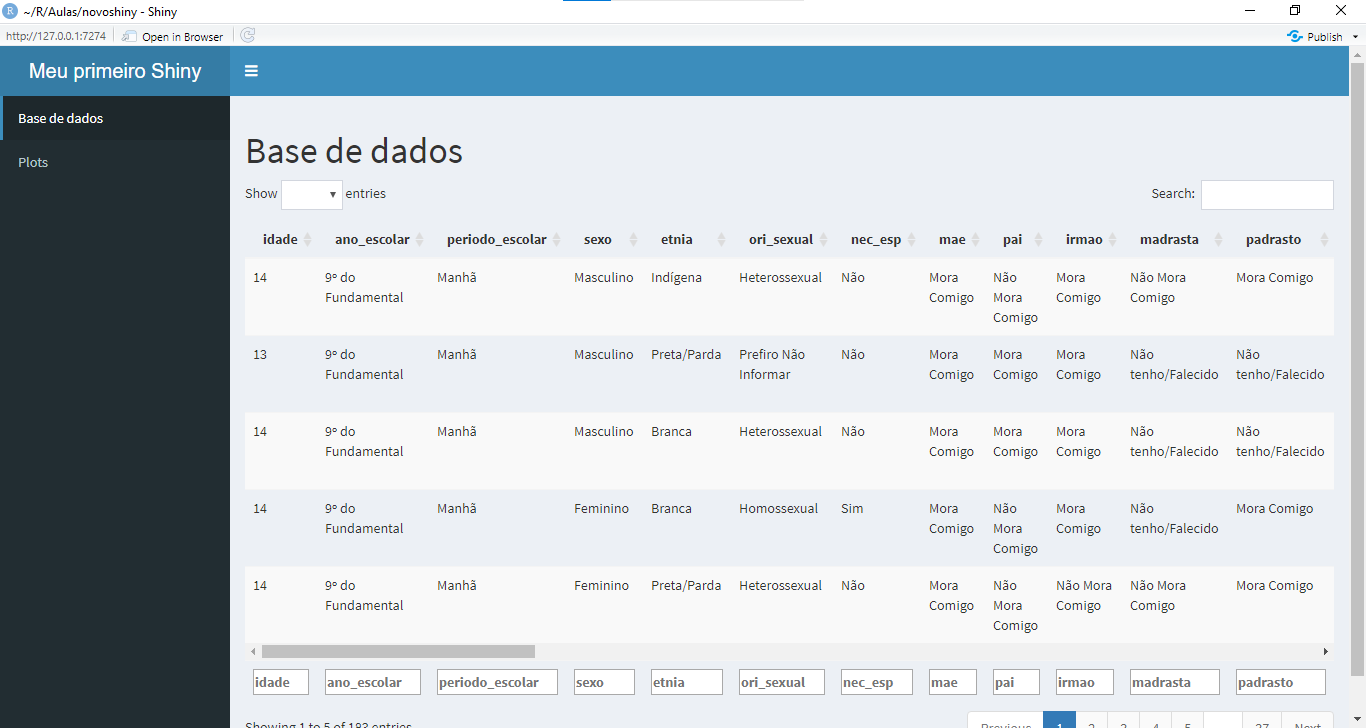
\includegraphics{./imagens/cap10imagem14.png}
\caption{menuItem Plots}
\end{figure}

  \bibliography{book.bib,packages.bib}

\end{document}
